% Structural refactor 2026-08-27. Empirical source: Team 7.
\chapter{Empirical Gold Dynamics: From Linear Models to Conditional Volatility}
\chapterstatus{Expanded reuse from Team 7 with an explicit two-layer data
boundary. Published AR/ARMA/ARIMA and regression tables retain the frozen 1
May 2006--31 December 2024 Yahoo sample. Descriptive, dependence,
distributional, GARCH and fractional-differencing figures are regenerated by
the unified branch from current LSE inputs; their aligned window is 5 January
2021--1 July 2026. The two layers are never merged silently.}

\section{Empirical Objective and Sample Boundary}

Chapter~2 explains why gold has to be read across monetary regimes. The present
chapter asks a narrower question: what can a conventional daily time-series
analysis learn from the historical sample before an option-implied,
continuous-time model is introduced? The sequence moves from returns and
cross-asset dependence to conditional-mean models, stylised facts and
conditional variance. It is diagnostic. It does not claim that historical
Yahoo observations, the current LSE macro panel and the later option surface
are one homogeneous dataset.

\section{Data and Econometric Framework}
\subsection{Return Construction}

A rigorous econometric analysis of gold and silver requires a clear and consistent definition
of asset returns. Throughout the paper we work with price time series observed at regular
intervals and transform these prices into simple and log returns in order to obtain
stationary, scale–free measures of performance that can be compared across assets and time
horizons (see, e.g., \sourcecitation{Wooldridge2020,Tsay2022}). All data work and empirical results in this paper are fully replicable using the
accompanying code and scripts provided in D'Amico and Weisz~\sourcecitation{SFClubPoliTo_GoldVolatilityCode}.
\subsubsection{Price series and notation}

Let $P^{(i)}_t$ denote the price of asset $i$ at time $t$, where $t = 1,2,\dots,T$ indexes
equally spaced observation dates (for example, daily or weekly trading days). In our
application, the set of assets $i$ includes gold, silver, an equity index, a government bond
benchmark, and a broad US dollar index.\footnote{The exact instruments and data sources
are specified in Section~\textit{Asset Selection: Bonds, Stocks, Dollar}.}
Working with prices directly is informative for descriptive purposes, but prices are typically 
non–stationary and depend on the scale of the asset. For econometric modeling we therefore
move to returns, which remove the level effect and produce a dimensionless measure of
percentage change \sourcecitation{Wooldridge2020}.
\subsubsection{Simple returns}

The starting point is the one–period simple gross return. For a given asset $i$, the gross
return between $t-1$ and $t$ is defined as
\[
1 + R^{(i)}_t = \frac{P^{(i)}_t}{P^{(i)}_{t-1}},
\]
so that $1 + R^{(i)}_t$ measures the growth factor of the price over a single period. 
Rearranging, we can write
\[
P^{(i)}_t = P^{(i)}_{t-1} (1 + R^{(i)}_t),
\]
which emphasizes that the current price is obtained by compounding the past price with the
realized return. The net simple return $R^{(i)}_t$ is then
\[
R^{(i)}_t = \frac{P^{(i)}_t - P^{(i)}_{t-1}}{P^{(i)}_{t-1}},
\]
representing the percentage change in the price between two consecutive observations.

Over multiple periods, from $t-k$ to $t$, the $k$–period simple gross return is defined as
\[
1 + R^{(i)}_{t,[k]} = \frac{P^{(i)}_t}{P^{(i)}_{t-k}}
= \prod_{j=0}^{k-1} \bigl(1 + R^{(i)}_{t-j}\bigr).
\]
This expression shows that multi–period gross returns are obtained by compounding the
sequence of one–period gross returns. Although intuitive, simple returns are not additive
over time, which complicates some aspects of statistical analysis and portfolio aggregation.
\subsubsection{Log returns and time additivity}

To address these limitations, it is standard in empirical finance and time–series analysis
to work with log (continuously compounded) returns \sourcecitation{Tsay2022}. For asset $i$, the log
return between $t-1$ and $t$ is defined as
\[
r^{(i)}_t = \ln \bigl(1 + R^{(i)}_t\bigr)
= \ln \left( \frac{P^{(i)}_t}{P^{(i)}_{t-1}} \right)
= \ln P^{(i)}_t - \ln P^{(i)}_{t-1},
\]
where we denote $p^{(i)}_t = \ln P^{(i)}_t$ the log price. Log returns preserve the ranking
of simple returns but possess a key technical advantage: they are additive over time. For a
$k$–period horizon we have
\[
r^{(i)}_{t,[k]}
= \ln \bigl(1 + R^{(i)}_{t,[k]}\bigr)
= \sum_{j=0}^{k-1} r^{(i)}_{t-j}.
\]
Thus the total log return over a holding period is simply the sum of the intermediate
one–period log returns. This time additivity greatly simplifies theoretical modeling and
empirical work, especially when aggregating returns across different horizons or computing
cumulative performance.

In addition, for small net returns $R^{(i)}_t$ in absolute value, the approximation
$r^{(i)}_t \approx R^{(i)}_t$ holds, so that log returns can be interpreted as approximate
percentage changes. For daily or weekly data on liquid financial assets, log returns retain
an intuitive economic interpretation while offering more tractable statistical properties
\sourcecitation{Tsay2022}.
\subsubsection{Choice of return measure in this study}

In line with the empirical literature on precious metals, we compute and analyze log
returns for all assets considered in the paper. Simple returns are used only for
intermediate computations and for robustness checks when comparing with existing studies
expressed in percentage terms. Concretely, given a price series $P^{(i)}_t$ for gold,
silver, bonds, equities, or the US dollar index, we define the corresponding log return
series by
\[
r^{(i)}_t = \ln P^{(i)}_t - \ln P^{(i)}_{t-1},
\]
and we treat $\{ r^{(i)}_t \}_{t=1}^T$ as the primary object of interest in the econometric
analysis that follows.

Working with log returns has two main implications for the rest of the paper: it facilitates the comparison of co–movements between gold, silver, and other financial
assets, since all series are expressed on a common, dimensionless scale and additionally provides a natural starting point for the time–series modeling in subsequent chapters, where we study distributional properties, temporal dependence, and conditional volatility
using models tailored to return dynamics.
\subsection{Asset Selection: Bonds, Stocks, Dollar}
The empirical analysis focuses on the joint behaviour of gold and silver with respect to
three major segments of global financial markets: government bonds, equities, and the US
dollar. This subsection describes the exact assets, indices, and data sources used in the
paper, as well as the sampling frequency and time span of the dataset.
\subsubsection{Precious metals}

As reference precious–metal assets we use the SPDR Gold Shares ETF (GLD) and the iShares Silver Trust (SLV), both quoted in US dollars and traded on U.S. exchanges. Gold is treated as the primary asset of interest, while silver provides a
natural benchmark to assess whether empirical properties and co–movements are specific to
gold or shared across precious metals. Using prices denominated in US dollars ensures
comparability with the chosen bond, equity, and currency variables, and avoids additional
complications arising from exchange–rate conversions. These highly liquid ETFs provide practical proxies for the spot prices of gold and silver over a long sample period.
\subsubsection{Government bonds}

For the fixed-income side, the current figure layer employs the LSE 10-year
U.S. Treasury yield (\texttt{US10Y}); the analysis uses daily yield changes.
The frozen Team~7 tables retain their original \texttt{\^TNX} construction.
\subsubsection{Equities}

Equity conditions in the current figure layer are represented by SPY, a
liquid ETF proxy for the S\&P~500. The frozen tables retain the original
\texttt{\^GSPC} index series.
\subsubsection{US dollar}

Currency conditions in the current figure layer use a transparent DXY-formula
proxy reconstructed from six LSE exchange rates: EUR/USD, USD/JPY, GBP/USD,
USD/CAD, USD/SEK and USD/CHF, with standard DXY exponents and normalization to
100 at the first aligned observation. It is not represented as the official
ICE DXY. The frozen Team~7 tables retain the original DX-Y.NYB proxy.
\subsubsection{Sampling frequency and sample period}

All series are sampled daily. The regenerated LSE panel contains 1,370 aligned
observations from 5 January 2021 to 1 July 2026; the end date is set by the
available \texttt{US10Y} history, while market and FX inputs extend to 26
August 2026. Published conditional-mean and regression tables below remain on
the separate 2006--2024 legacy window.

Table~\ref{tab:t7-descriptive-statistics} restores the complete descriptive
panel reported in the Team~7 article. The Treasury series is a daily yield
change rather than an asset return, so its scale must not be compared directly
with the ETF and index returns.

\begin{table}[htbp]
\centering
\caption{Descriptive statistics for the synchronized Team~7 sample}
\label{tab:t7-descriptive-statistics}
\small
\resizebox{\textwidth}{!}{%
\begin{tabular}{lrrrrrrrr}
\toprule
Series & $N$ & Mean & Std. dev. & Min. & Q1 & Median & Q3 & Max. \\
\midrule
Gold (GLD)           & 4,694 &  0.0003 & 0.0111 & -0.0919 & -0.0052 &  0.0005 & 0.0060 & 0.1070 \\
Silver (SLV)         & 4,694 &  0.0001 & 0.0199 & -0.1983 & -0.0087 &  0.0007 & 0.0099 & 0.1347 \\
S\&P 500             & 4,694 &  0.0003 & 0.0124 & -0.1277 & -0.0041 &  0.0007 & 0.0058 & 0.1096 \\
U.S. Dollar Index    & 4,694 &  0.0000 & 0.0048 & -0.0272 & -0.0026 &  0.0000 & 0.0027 & 0.0252 \\
10-year yield change & 4,694 & -0.0001 & 0.0577 & -0.4700 & -0.0330 & -0.0020 & 0.0330 & 0.3320 \\
\bottomrule
\end{tabular}}
\begin{minipage}{0.96\textwidth}
\footnotesize\emph{Notes:} Daily log returns are used for GLD, SLV, the
S\&P~500 and DXY; the last row reports the daily change in the 10-year U.S.
Treasury yield. Sample: 1 May 2006--31 December 2024.
\end{minipage}
\end{table}


Overall, the mean daily returns are close to zero for all assets, as expected at this
frequency, while standard deviations differ markedly across series. Silver (SLV) and the
S\&P 500 display the highest volatility, whereas the U.S. dollar index and changes in the
10-year yield are substantially less volatile in relative terms. The minima and maxima
suggest that all series occasionally experience large daily moves, with more pronounced
extremes for silver and equities, anticipating the heavy tails and volatility clustering
documented in later chapters.
\subsection{Correlation and Regression Design}

The empirical framework of this paper is built around two complementary tools: correlation
measures and linear regression models. Correlations provide a first description of the
co–movements between gold, silver, and other financial assets, while regressions formalize
these relationships in a conditional, ceteris paribus sense and allow us to control for
multiple drivers simultaneously. In this subsection we outline the design choices behind
these tools, setting the stage for the econometric analysis developed in the following
chapter.
\subsubsection{Static and dynamic correlations}

Let $r^{(i)}_t$ and $r^{(j)}_t$ denote the log returns of two assets $i$ and $j$ at time $t$,
constructed as described in the previous subsections. A natural measure of linear
dependence between the two series is the Pearson correlation coefficient
\[
\rho_{ij} = \frac{\operatorname{Cov}(r^{(i)}_t, r^{(j)}_t)}
{\sqrt{\operatorname{Var}(r^{(i)}_t)\,\operatorname{Var}(r^{(j)}_t)}},
\]
which summarizes whether returns tend to move in the same direction ($\rho_{ij} > 0$),
in opposite directions ($\rho_{ij} < 0$), or show no linear association ($\rho_{ij} \approx 0)$.
Under the usual assumptions of weak stationarity, correlations can be estimated consistently
from the sample and provide a compact description of average co–movement over the whole
sample period (see, e.g., standard treatments in time–series econometrics).

However, financial markets are characterized by changing regimes and time–varying
dependence. To account for this, we complement static correlations with \emph{rolling}
correlations computed over moving windows. Given a window length $W$, the rolling
correlation between assets $i$ and $j$ at time $t$ is defined as the sample correlation
computed using only the observations $t-W+1,\dots,t$. By sliding the window along the
sample, we obtain a time series of correlation estimates that reveals how the strength and
sign of co–movements evolve across tranquil periods and episodes of market stress.

In our context, static correlations offer a baseline picture of how gold and silver are
related to bonds, equities, and the US dollar on average, while rolling correlations
highlight whether gold behaves more like a hedge or a safe haven in specific subperiods,
such as financial crises or high–inflation episodes.

In the empirical implementation, we first compute the static Pearson correlation matrix
using the daily return and yield–change series over the full common sample period. This
matrix provides a compact summary of the average linear co–movements between gold, silver,
bonds, equities and the U.S. dollar.

\begin{figure}[htbp]
\centering
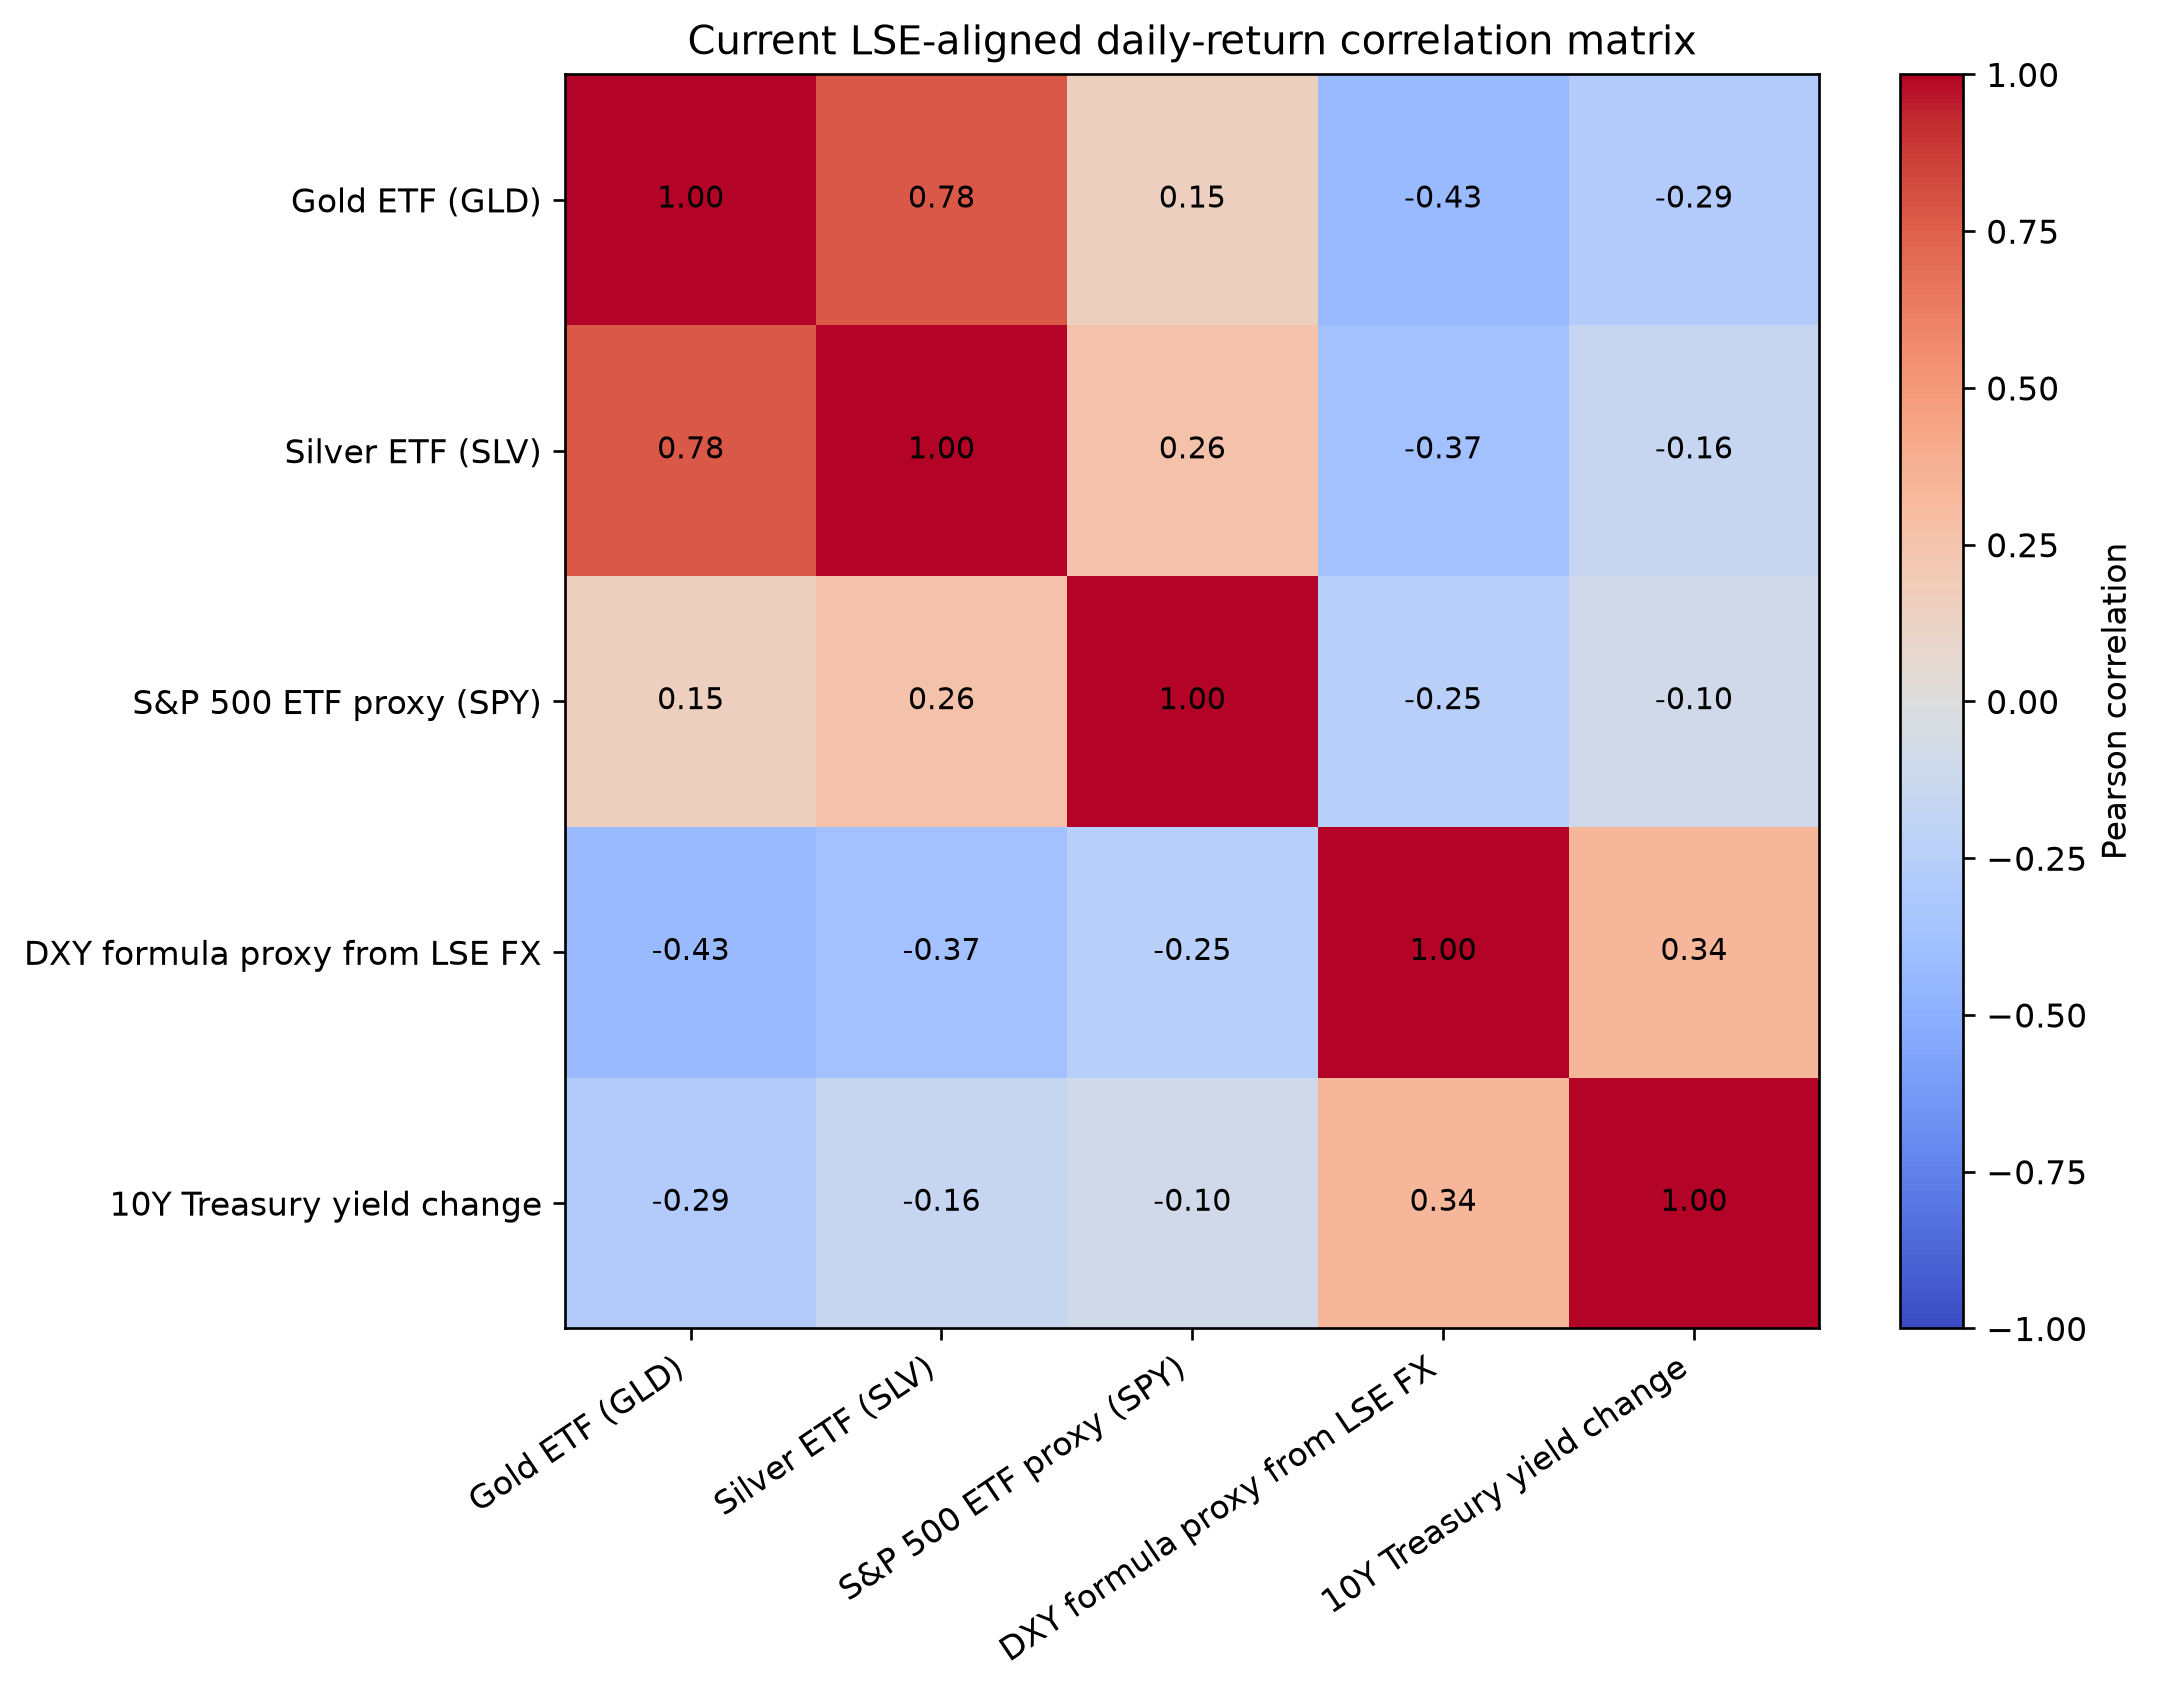
\includegraphics[width=0.82\textwidth]{img/team7_empirical/correlation_heatmap.png}
\caption{Static correlation matrix for the synchronized daily sample}
\label{fig:t7-correlation-heatmap}
\end{figure}

The current LSE matrix in Figure~\ref{fig:t7-correlation-heatmap} reveals
several patterns. GLD and SLV exhibit a strong positive correlation ($0.78$).
GLD is weakly correlated with SPY ($0.15$), while its correlations with the
DXY-formula proxy ($-0.43$) and the change in the 10-year Treasury yield
($-0.29$) are negative. SLV has a larger positive SPY correlation ($0.26$), a
negative dollar-proxy correlation ($-0.37$), and a weaker yield-change
correlation ($-0.16$). These are unconditional sample
associations, not universal hedge coefficients; the rolling evidence below
shows that both sign and magnitude vary through time.
\subsubsection{Linear regression framework}


Building on the correlation analysis discussed above, we next specify linear regression models that relate gold and silver returns to the macro-financial drivers identified in Chapter~2 and formalised econometrically in Chapter~5.
While correlations are symmetric and purely descriptive, regression models impose a
direction of explanation and allow us to condition on multiple variables at once
\sourcecitation{Wooldridge2020}. Following the econometric framework introduced in the theoretical
section on ordinary least squares, we model gold and silver returns as linear functions of
bond, equity, and dollar returns:
\[
r^{gold}_t = \beta_0 + \beta_1 r^{bond}_t + \beta_2 r^{equity}_t
+ \beta_3 r^{usd}_t + u_t,
\]
\[
r^{silver}_t = \gamma_0 + \gamma_1 r^{bond}_t + \gamma_2 r^{equity}_t
+ \gamma_3 r^{usd}_t + v_t,
\]
where $u_t$ and $v_t$ denote error terms capturing all other factors that affect precious–
metal returns but are not explicitly included in the specification. These baseline models
allow us to quantify how gold and silver co–move with fixed–income markets, stock markets,
and the US dollar, holding the other drivers constant.

From a conceptual standpoint, the interpretation of the coefficients can follow two
complementary perspectives. A \emph{causal} interpretation would require strong identifying
assumptions on the error terms and on the absence of omitted variables, as emphasized in
the discussion of the zero conditional mean assumption and omitted variable bias in the
OLS framework. In this paper, we primarily adopt a \emph{predictive} and descriptive
perspective: the coefficients are interpreted as measures of conditional co–movement and as
indicators of hedge and safe–haven properties, rather than as structural causal effects
(see also the distinction between causal and forecasting objectives in standard
econometrics and time–series texts, e.g., \sourcecitation{Wooldridge2020,Tsay2022}).
\subsubsection{Extensions and robustness}

The original article presented volatility modelling as a future extension. In
the unified thesis, part of that agenda is already completed: GARCH evidence is
reported later in this chapter, continuous-time stochastic variance and jumps
are developed in Chapter~8, and option-surface calibration is performed in
Chapter~9. Additional regressors, quantile methods and formal regime or causal
identification remain robustness extensions rather than completed results.

The linear regression framework adopted in this chapter is primarily designed for descriptive and predictive purposes rather than for structural causal inference. The estimated coefficients should therefore be interpreted as measures of conditional comovement and as indicative of hedge or safe-haven behaviour \emph{in our sample and at the daily frequency considered}, under the maintained assumptions on the error term and the chosen set of regressors, rather than as evidence of deep causal effects.


These design choices provide a coherent link between the descriptive correlation analysis,
the linear regression framework, and the volatility models that follow. The following
sections implement this framework empirically, estimating the models for gold and silver
and interpreting the results in light of their proposed roles as hedges, safe havens, and
diversifiers.


\section{Applied Cross-Asset Evidence}

Static correlations conceal economically important changes in sign and
magnitude. Figure~\ref{fig:t7-gold-rolling-correlations} regenerates the three
GLD rolling-correlation series from the current LSE panel. The dollar relation is
predominantly negative, whereas the equity and yield-change relations are more
state dependent. No rolling correlation alone identifies a causal channel.

\begin{figure}[htbp]
\centering
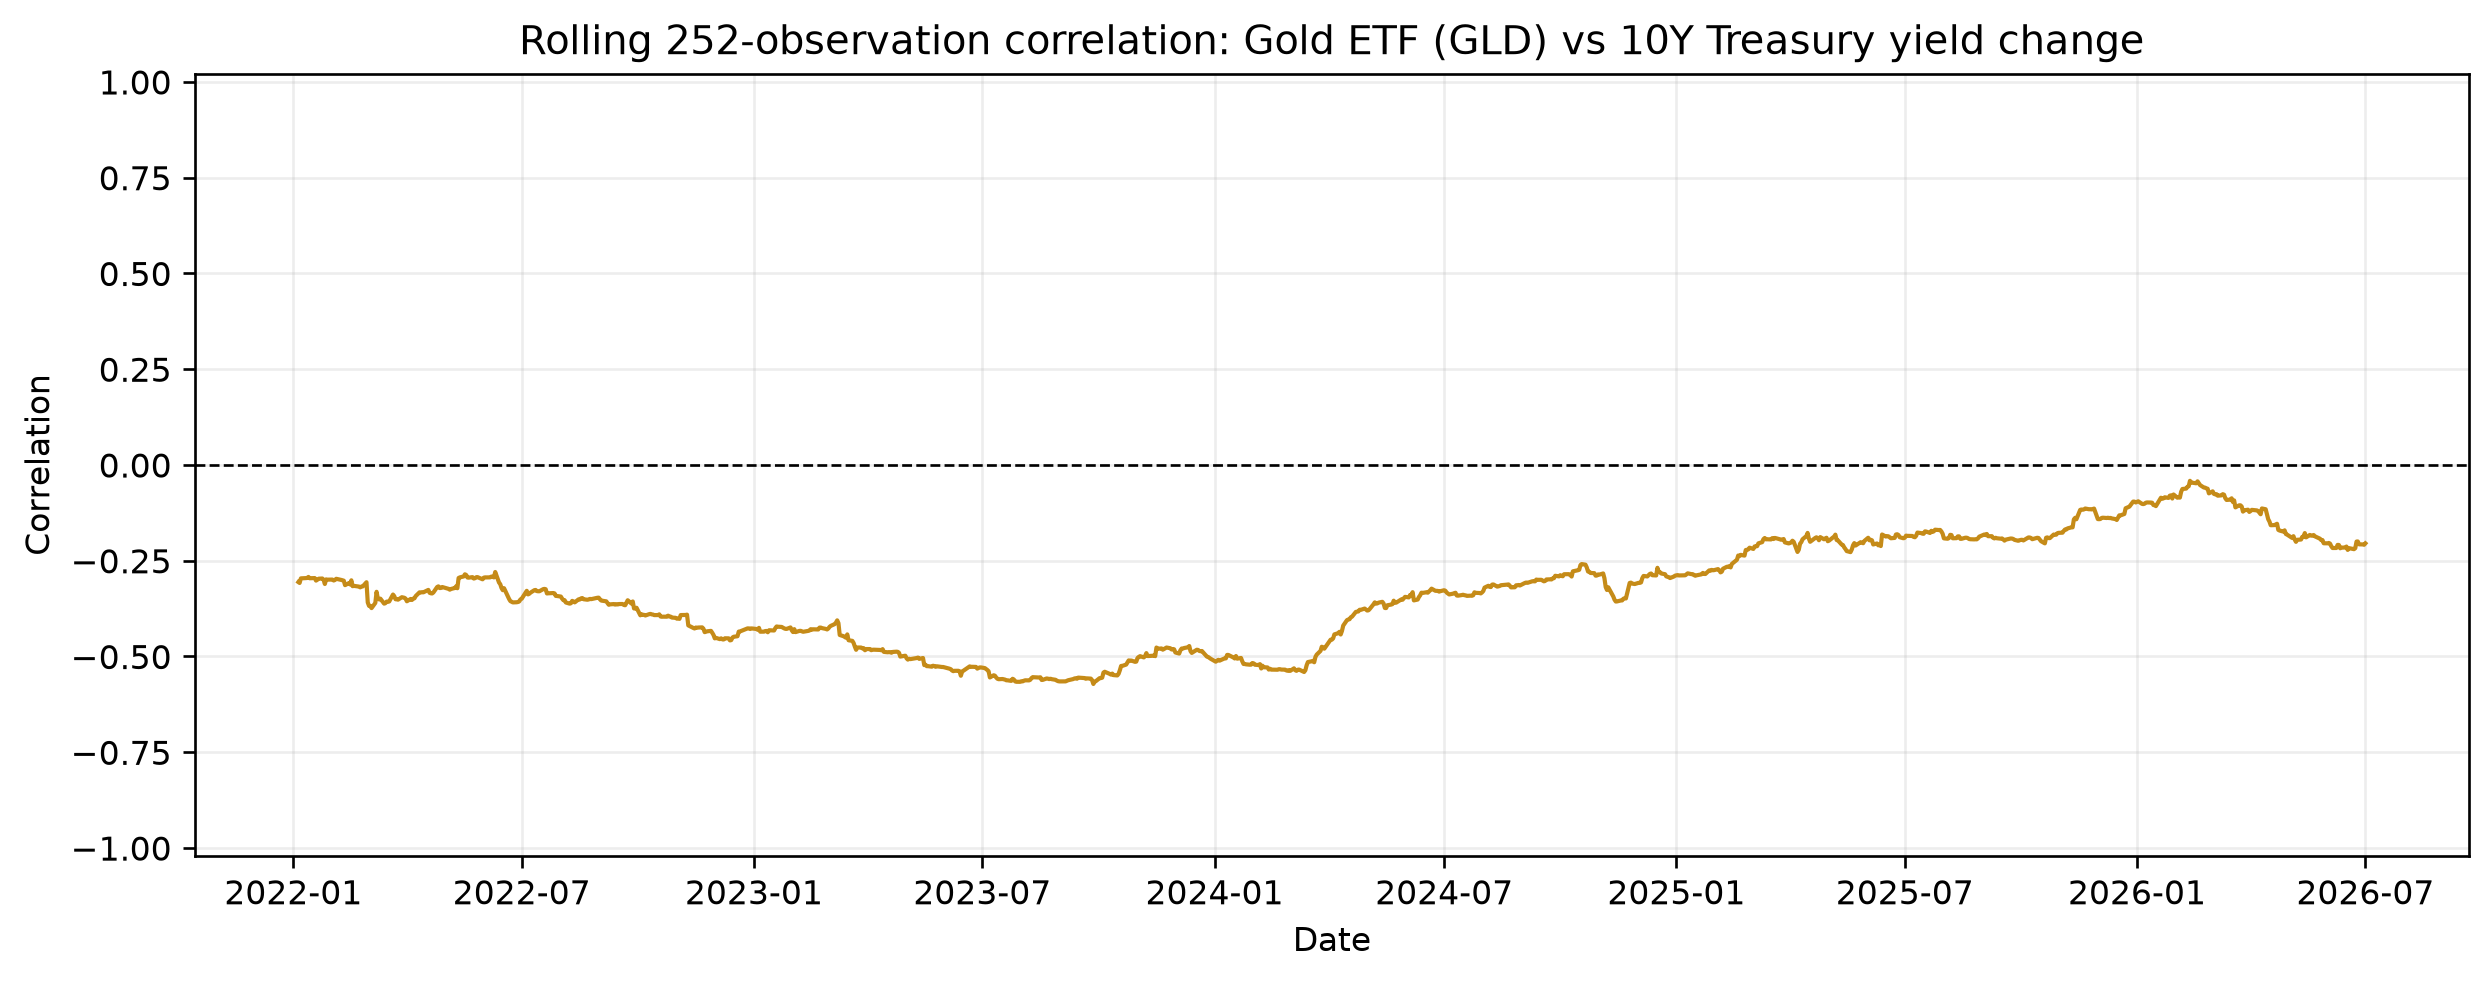
\includegraphics[width=0.88\textwidth]{img/team7_empirical/rolling_corr_gold_ust10y.png}
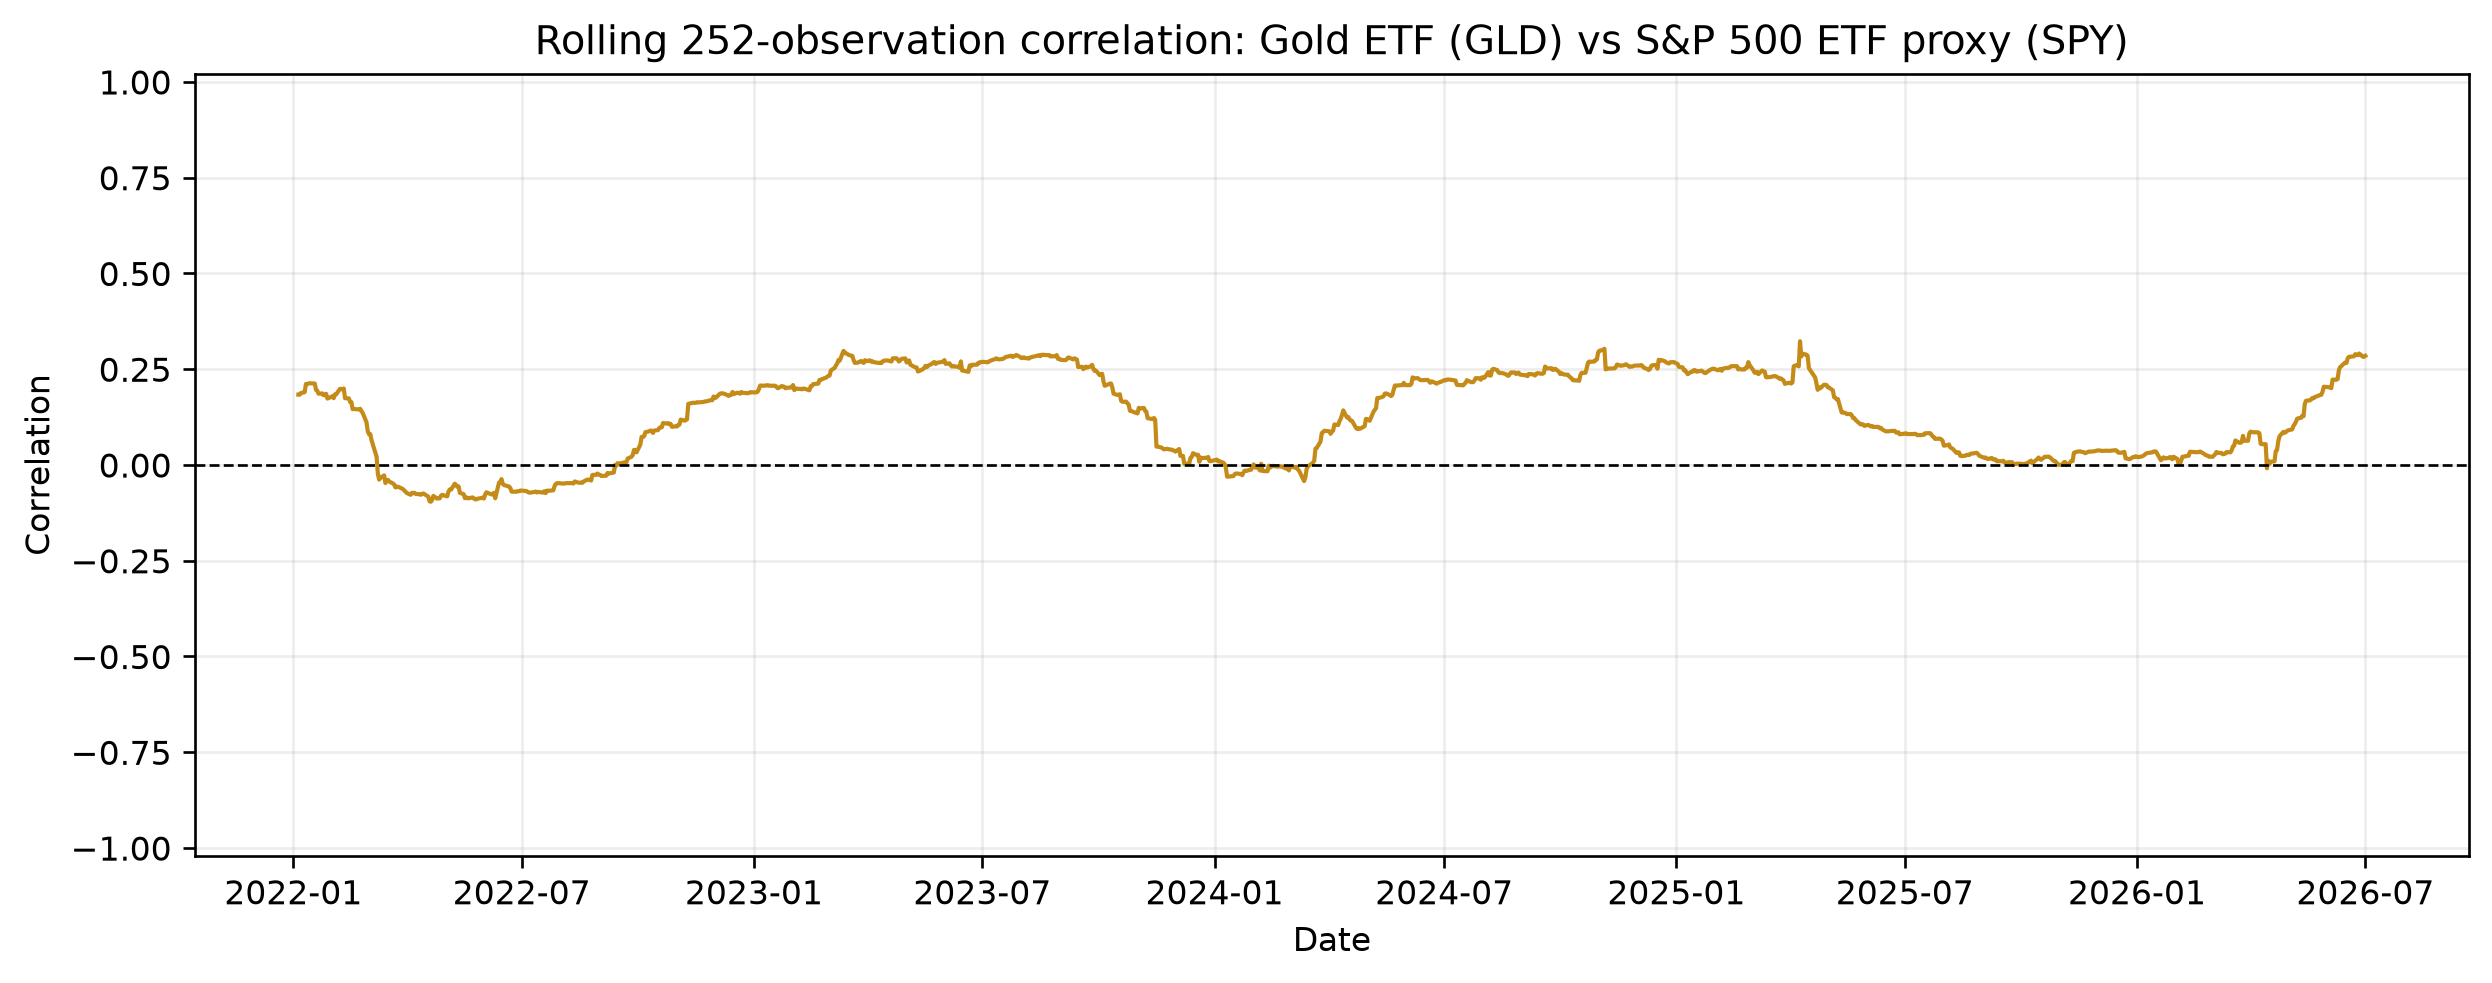
\includegraphics[width=0.88\textwidth]{img/team7_empirical/rolling_corr_gold_sp500.png}
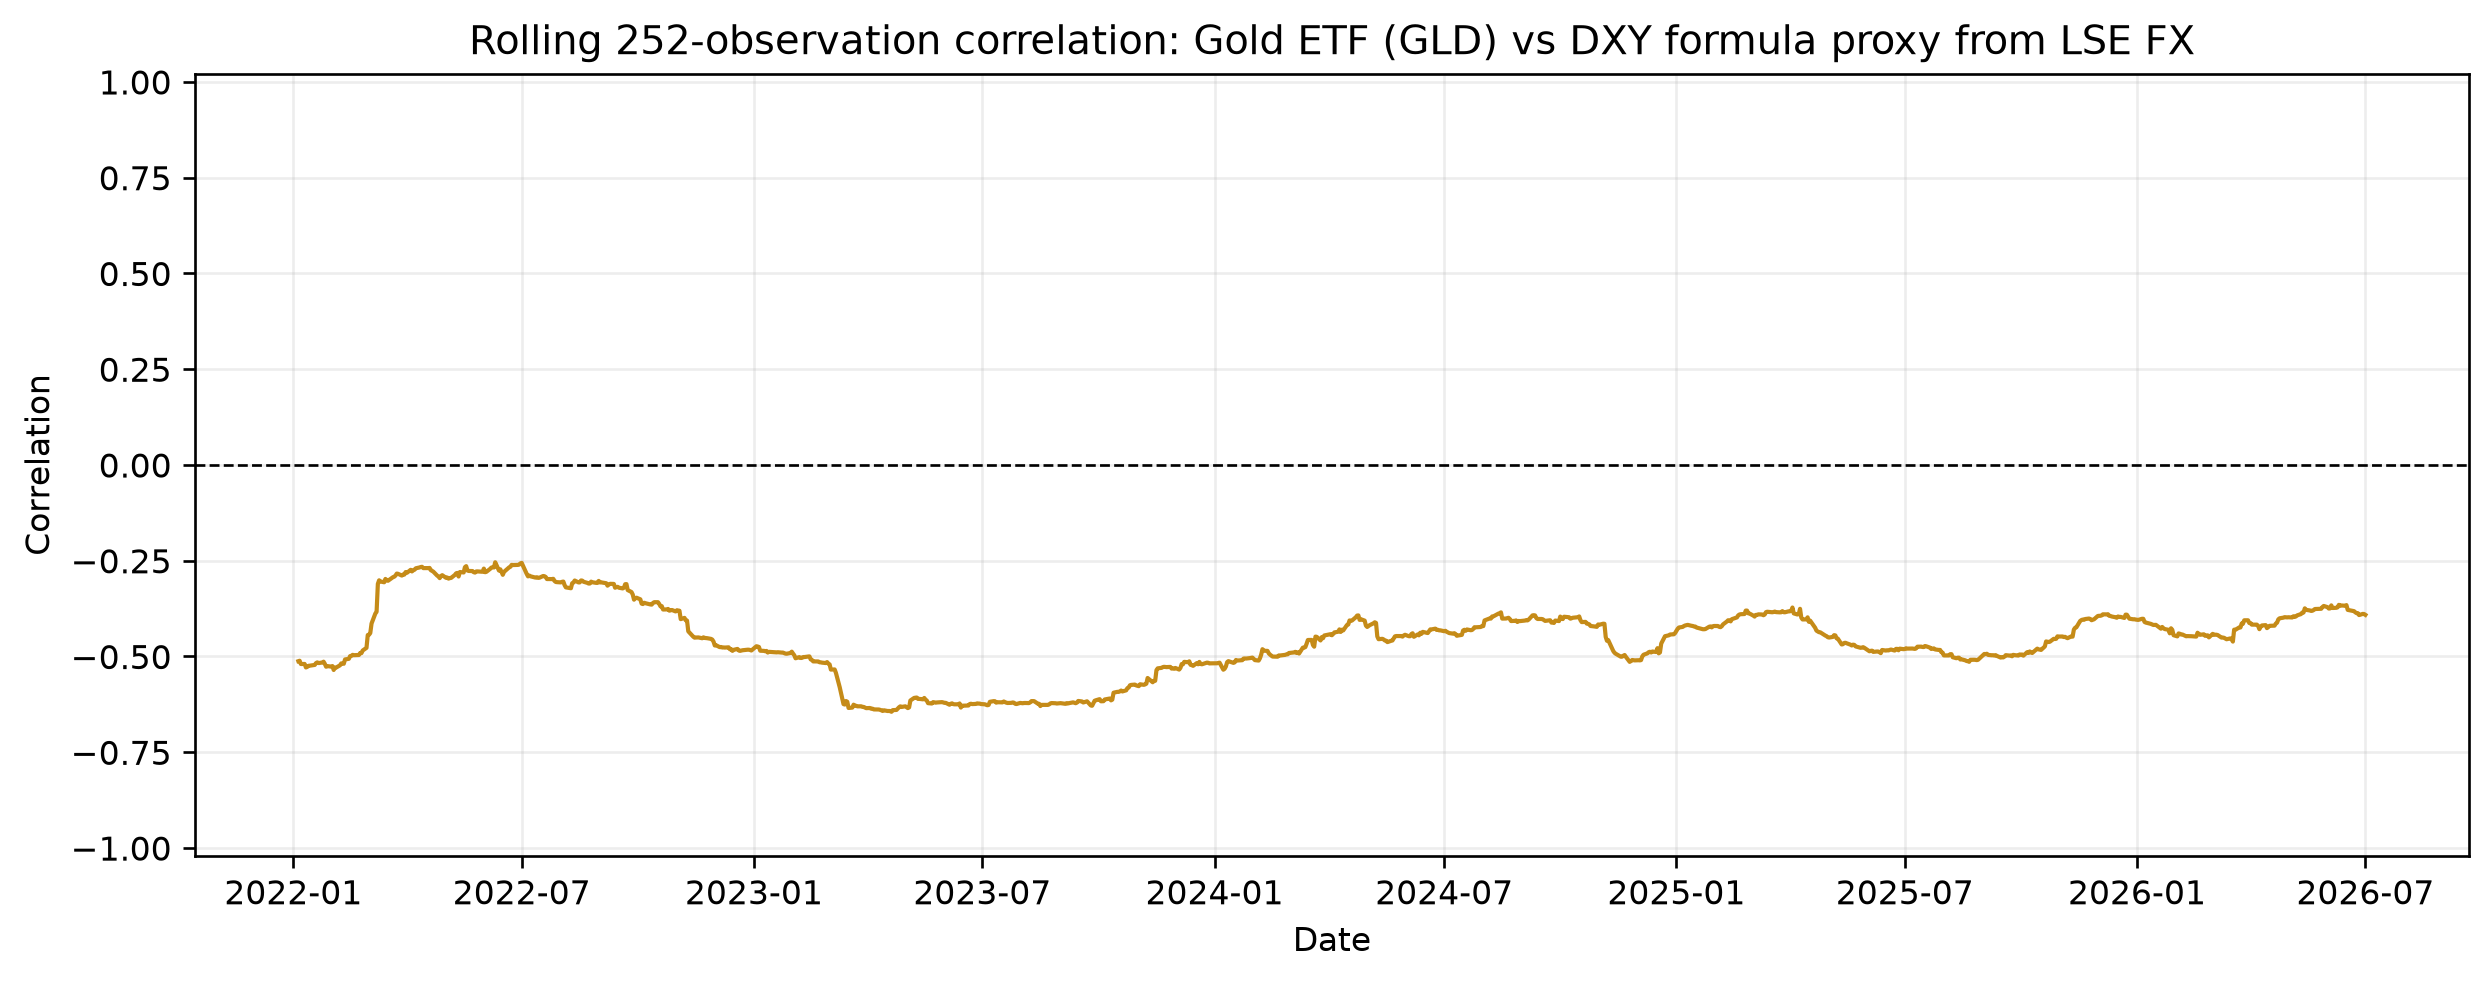
\includegraphics[width=0.88\textwidth]{img/team7_empirical/rolling_corr_gold_dxy.png}
\caption{Rolling 252-observation correlations of GLD returns with LSE
Treasury-yield changes, SPY returns and the transparent DXY-formula proxy}
\label{fig:t7-gold-rolling-correlations}
\end{figure}

The regression estimates in Table~\ref{tab:t7-gold-ols} quantify these
associations. Individually, gold loads negatively on yield changes and DXY;
the single-factor equity coefficient is small and positive. In the joint
specification, the DXY and yield-change coefficients remain statistically
different from zero, while the equity coefficient does not. The dollar factor
accounts for most of the reported explanatory power.

\begin{table}[htbp]
\centering
\caption{Gold-return regressions in the Team~7 sample}
\label{tab:t7-gold-ols}
\small
\begin{tabular}{lrrrr}
\toprule
 & Yield only & Equity only & Dollar only & Joint \\
\midrule
Yield change & $-0.0375^{***}$ & --- & --- & $-0.0292^{***}$ \\
             & $(0.0039)$      &     &     & $(0.0036)$       \\
S\&P 500 return & --- & $0.0506^{**}$ & --- & $0.0224$ \\
                &     & $(0.0250)$    &     & $(0.0250)$ \\
DXY return   & --- & --- & $-0.9810^{***}$ & $-0.9248^{***}$ \\
             &     &     & $(0.0450)$       & $(0.0466)$       \\
Constant     & $0.0003^{*}$ & $0.0003$ & $0.0003^{**}$ & $0.0003^{**}$ \\
             & $(0.0002)$   & $(0.0002)$& $(0.0001)$    & $(0.0001)$    \\
\midrule
$N$          & 4,694 & 4,694 & 4,694 & 4,694 \\
$R^2$        & 0.038 & 0.003 & 0.176 & 0.197 \\
Adjusted $R^2$ & 0.0376 & 0.0026 & 0.1760 & 0.1961 \\
\bottomrule
\end{tabular}
\begin{minipage}{0.92\textwidth}
\footnotesize\emph{Notes:} Heteroskedasticity-robust HC1 standard errors in
parentheses. $^{*}p<0.10$, $^{**}p<0.05$, $^{***}p<0.01$.
\end{minipage}
\end{table}

Silver provides a useful comparator rather than a substitute for gold. Its
rolling relations in Figure~\ref{fig:t7-silver-rolling-correlations} are more
equity-sensitive and remain time varying. In the joint regressions, silver's
equity loading is $0.2625$ (robust standard error $0.0424$), compared with
$0.0224$ ($0.0250$) for gold; the dollar loadings are $-1.6229$ ($0.0860$)
and $-0.9248$ ($0.0466$), respectively. The joint $R^2$ values are $0.205$
for silver and $0.197$ for gold.

\begin{table}[htbp]
\centering
\caption{Silver-return regressions in the Team~7 sample}
\label{tab:t7-silver-ols}
\small
\begin{tabular}{lrrrr}
\toprule
 & Yield only & Equity only & Dollar only & Joint \\
\midrule
Yield change & $-0.0206^{***}$ & --- & --- & $-0.0201^{***}$ \\
             & $(0.0067)$      &     &     & $(0.0062)$       \\
S\&P 500 return & --- & $0.3543^{***}$ & --- & $0.2625^{***}$ \\
                &     & $(0.0408)$     &     & $(0.0424)$       \\
DXY return   & --- & --- & $-1.7854^{***}$ & $-1.6229^{***}$ \\
             &     &     & $(0.0789)$        & $(0.0860)$        \\
Constant     & $0.0001$ & $0.0000$ & $0.0002$ & $0.0001$ \\
             & $(0.0002)$& $(0.0003)$& $(0.0002)$& $(0.0002)$ \\
\midrule
$N$          & 4,694 & 4,694 & 4,694 & 4,694 \\
$R^2$        & 0.004 & 0.049 & 0.182 & 0.205 \\
Adjusted $R^2$ & 0.0030 & 0.0485 & 0.1810 & 0.2050 \\
\bottomrule
\end{tabular}
\begin{minipage}{0.92\textwidth}
\footnotesize\emph{Notes:} Heteroskedasticity-robust HC1 standard errors in
parentheses. $^{*}p<0.10$, $^{**}p<0.05$, $^{***}p<0.01$.
\end{minipage}
\end{table}

\begin{figure}[htbp]
\centering
\begin{minipage}{0.49\textwidth}
\centering
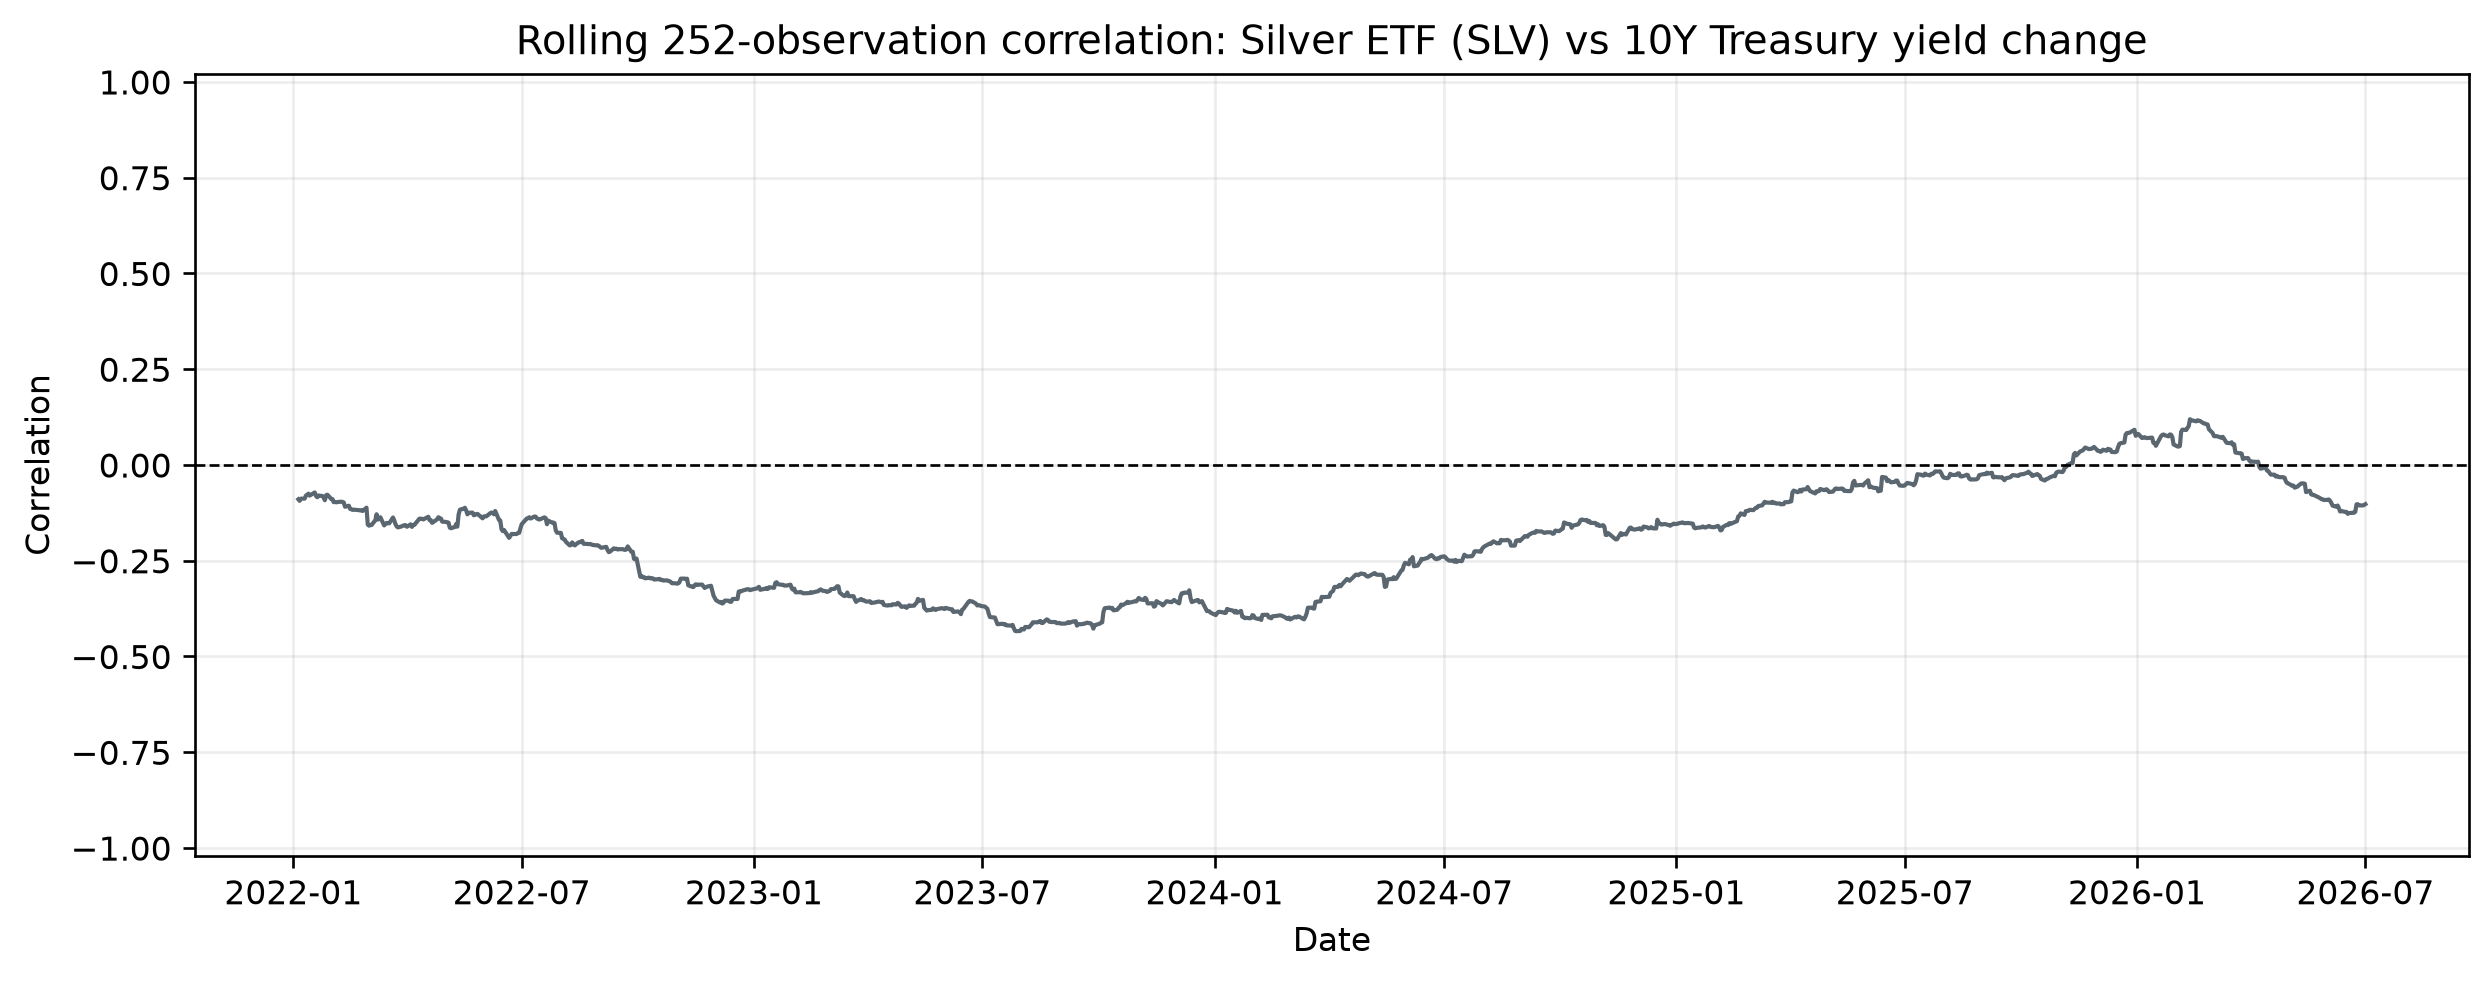
\includegraphics[width=\linewidth]{img/team7_empirical/rolling_corr_silver_ust10y.png}
\end{minipage}\hfill
\begin{minipage}{0.49\textwidth}
\centering
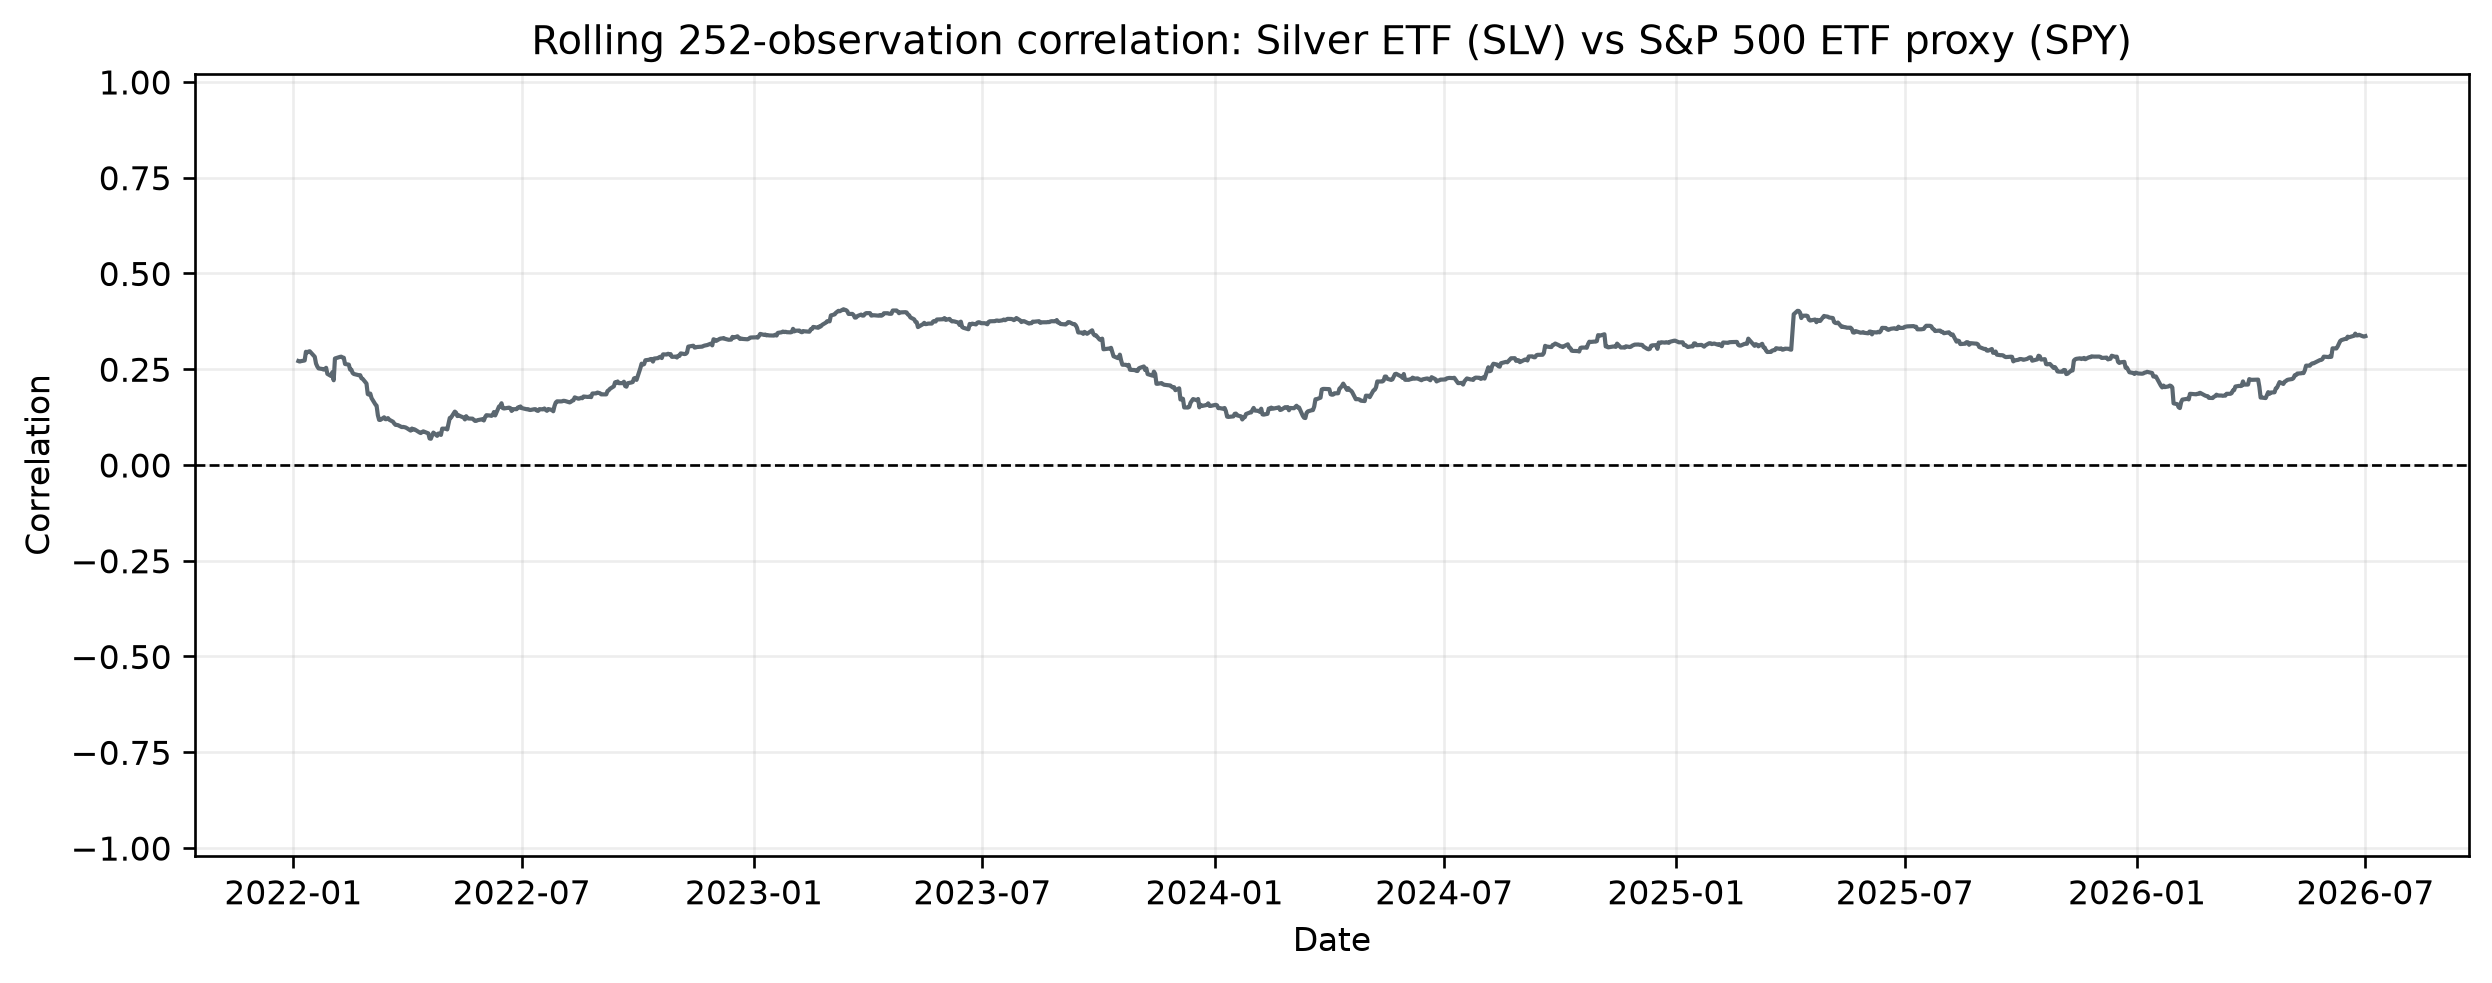
\includegraphics[width=\linewidth]{img/team7_empirical/rolling_corr_silver_sp500.png}
\end{minipage}

\begin{minipage}{0.55\textwidth}
\centering
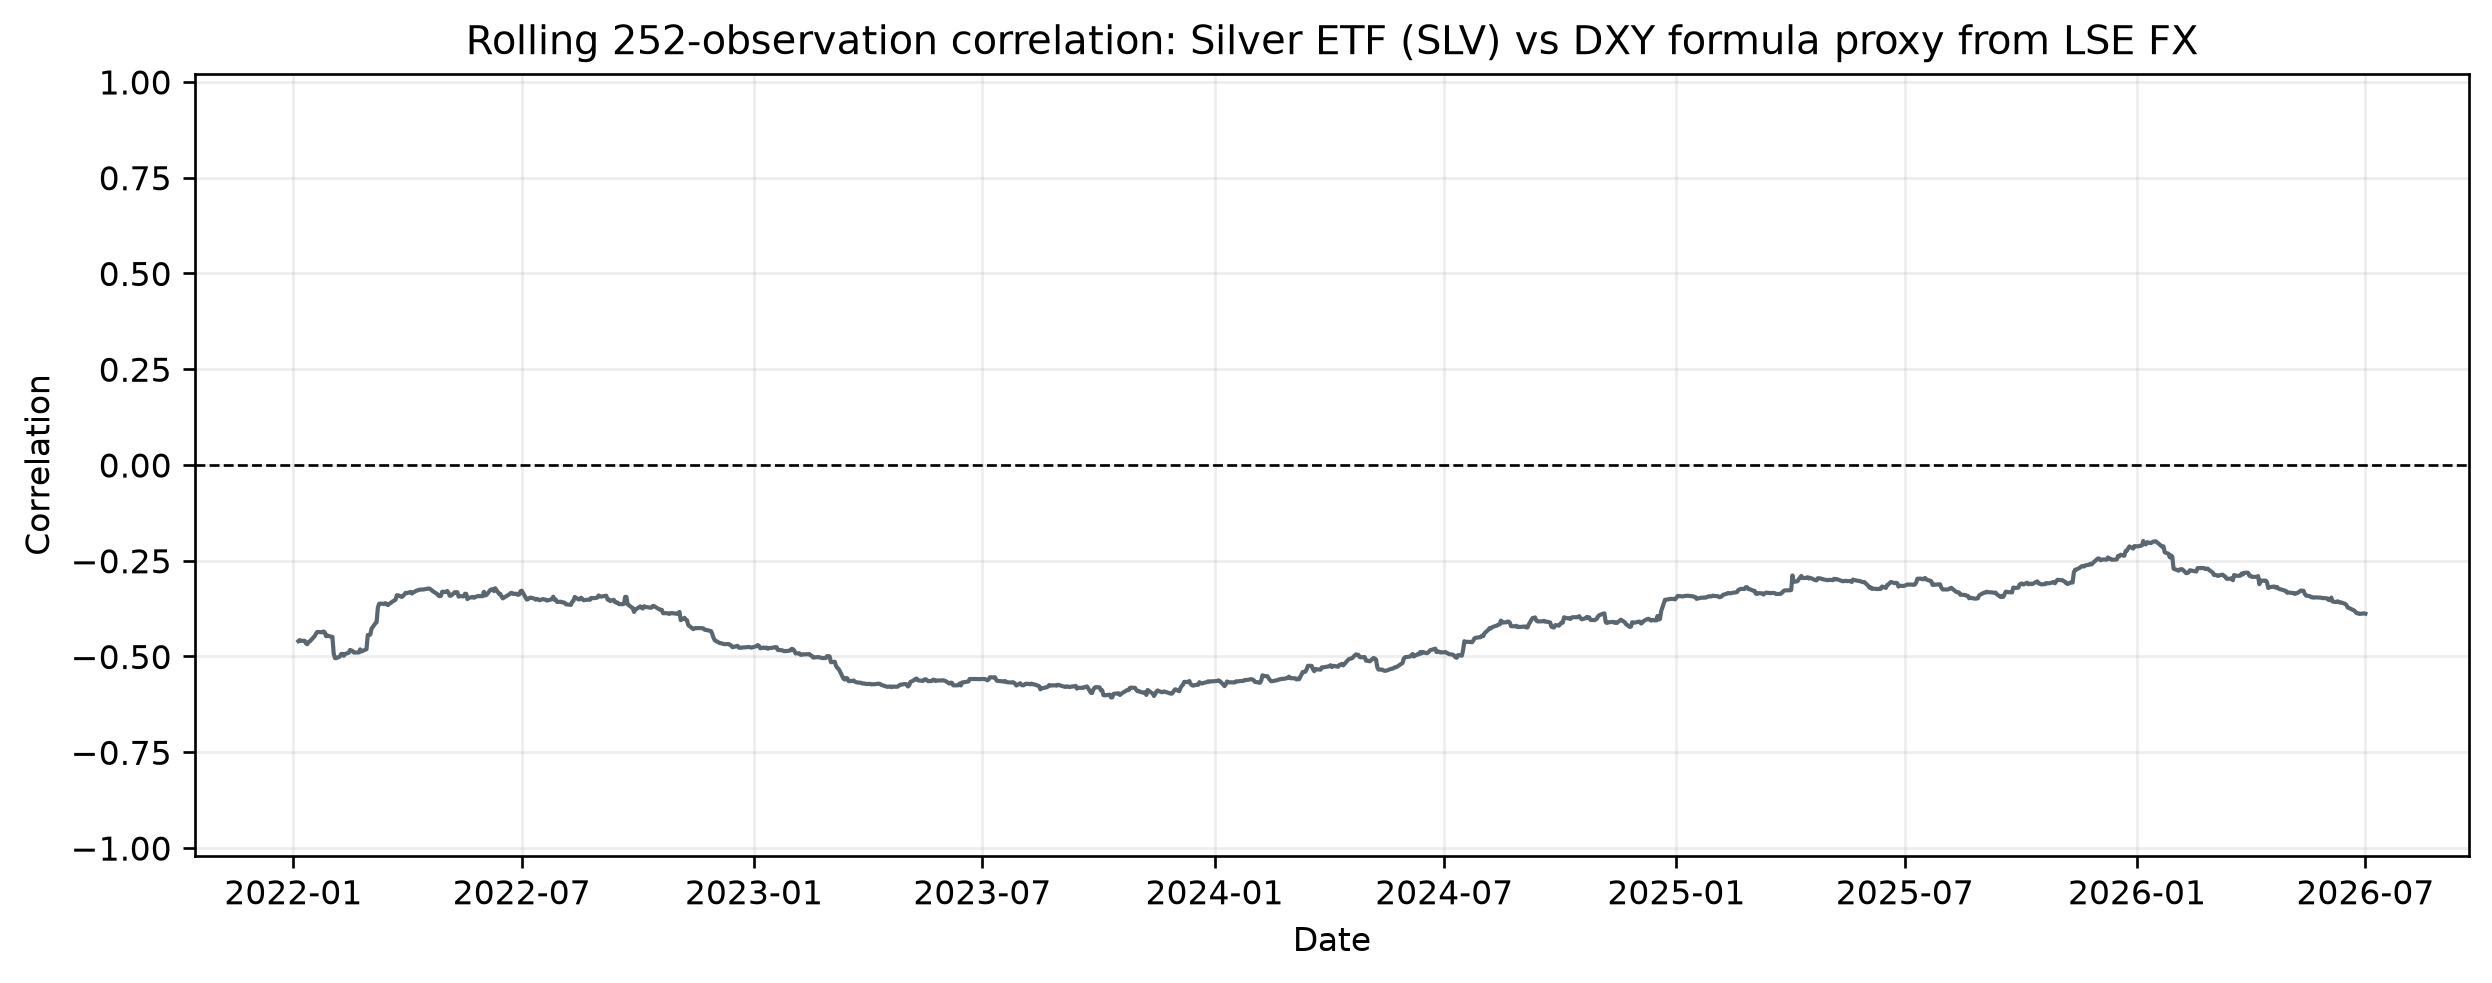
\includegraphics[width=\linewidth]{img/team7_empirical/rolling_corr_silver_dxy.png}
\end{minipage}
\caption{Rolling 252-observation correlations of SLV returns with LSE
Treasury-yield changes, SPY returns and the transparent DXY-formula proxy}
\label{fig:t7-silver-rolling-correlations}
\end{figure}

The combined evidence supports three limited conclusions. Gold and silver are
strongly related but silver is materially more volatile; gold's unconditional
equity relationship is weak; and the negative dollar relationship is much
more stable than the bond-yield or equity relations. The evidence motivates
state-dependent volatility modelling, but it does not establish a universal
safe-haven law.

\section{Log Prices, Returns and Stationarity}

The distinction between log-price levels and log returns governs the model
choice. Log prices are highly persistent and empirically close to a unit-root
process, whereas daily returns are much closer to weak stationarity. An AR(1)
fit to price levels consequently produces coefficients near one and very high
in-sample explanatory power: approximately $0.9993$ for gold with
$R^2\approx0.999$, and $0.9978$ for silver with $R^2\approx0.996$. These values
primarily record persistence and must not be read as useful economic
forecastability.

For returns, the same benchmark changes sharply. The estimated AR(1)
coefficient is approximately $-0.0024$ for gold and $0.0063$ for silver, with
robust standard errors near $0.0202$ and $0.0227$ and essentially zero
$R^2$. At the daily frequency the conditional mean is therefore weak even
though the price level is persistent.

\begin{table}[htbp]
\centering
\caption{AR(1) contrast between log-price levels and daily returns}
\label{tab:t7-ar1-level-return}
\small
\begin{tabular}{llrrrr}
\toprule
Asset & Dependent series & $\hat\phi_1$ & Robust s.e. & $t$-statistic & $R^2$ \\
\midrule
Gold   & Log price & 0.9993  & 0.0006 & 1653.18 & 0.9987 \\
Silver & Log price & 0.9978  & 0.0012 &  802.26 & 0.9956 \\
Gold   & Return    &-0.0024  & 0.0202 &   -0.12 & 0.0000 \\
Silver & Return    & 0.0063  & 0.0227 &    0.28 & 0.0000 \\
\bottomrule
\end{tabular}
\begin{minipage}{0.90\textwidth}
\footnotesize\emph{Notes:} Values reproduce the published Team~7 article
snapshot. High fit in levels reflects near-unit-root persistence, not reliable
return predictability.
\end{minipage}
\end{table}

\section{AR, ARMA and ARIMA Diagnostics}

Higher-order autoregressions do not overturn the AR(1) result. AIC and BIC
select low-dimensional specifications and the joint lag tests provide little
evidence that lagged daily returns explain current returns. ARMA searches also
remain parsimonious and are not stable enough across criteria to reveal a
substantive conditional-mean law.

\begin{table}[htbp]
\centering
\caption{Higher-order autoregressive diagnostics for daily returns}
\label{tab:t7-arp-diagnostics}
\small
\begin{tabular}{lrrrrr}
\toprule
Asset & AIC lag & BIC lag & $R^2$ & Joint $F$ & $p$-value \\
\midrule
Gold   & 1 & 1 & 0.000006 & 0.0144 & 0.9046 \\
Silver & 1 & 1 & 0.000040 & 0.0779 & 0.7801 \\
\bottomrule
\end{tabular}
\end{table}

ARIMA is not rejected because prices are non-stationary: differencing is
precisely how the model addresses that feature. On log prices, the legacy
selection produces ARIMA$(2,1,0)$ by AIC and ARIMA$(0,1,1)$ by BIC for gold;
for silver both criteria select ARIMA$(1,1,0)$. Once differenced, these models
are close to the simple ARMA descriptions of returns and add little predictive
structure at the horizon considered.

\begin{table}[htbp]
\centering
\caption{Information-criterion selections for ARMA returns and ARIMA log prices}
\label{tab:t7-arma-arima-selection}
\small
\begin{tabular}{lllrr}
\toprule
Asset & Series and criterion & Selected order & AIC & BIC \\
\midrule
Gold   & Return, AIC      & ARMA$(2,0)$  & -28,909.4140 & --- \\
Gold   & Return, BIC      & ARMA$(0,1)$  & --- & -28,889.9939 \\
Silver & Return, AIC/BIC  & ARMA$(1,0)$  & -23,448.9424 & -23,429.5802 \\
Gold   & Log price, AIC   & ARIMA$(2,1,0)$ & -28,909.4140 & --- \\
Gold   & Log price, BIC   & ARIMA$(0,1,1)$ & --- & -28,889.9939 \\
Silver & Log price, AIC/BIC & ARIMA$(1,1,0)$ & -23,448.9424 & -23,429.5802 \\
\bottomrule
\end{tabular}
\begin{minipage}{0.94\textwidth}
\footnotesize\emph{Notes:} The equality of several ARMA and ARIMA criteria is
expected because first-differenced log prices are the return series. Dashes
mark the criterion not used for the stated selection.
\end{minipage}
\end{table}

\section{Heavy Tails, Clustering and Persistence}

The return distribution shifts attention from the conditional mean to the
second moment and the tails. In the frozen 2006--2024 table layer, daily standard deviation
is approximately $1.1\%$ for gold and $2.0\%$ for silver. Estimated skewness is
about $-0.33$ and $-0.85$, while excess kurtosis is approximately $6.25$ and
$7.79$. Gaussian innovations therefore understate the frequency and asymmetry
of large moves, especially for silver.

\begin{table}[htbp]
\centering
\caption{Distributional moments of daily precious-metal returns}
\label{tab:t7-return-moments}
\small
\begin{tabular}{lrrrrr}
\toprule
Asset & Mean & Std. dev. & Skewness & Excess kurtosis & Kurtosis \\
\midrule
Gold   & 0.00028 & 0.01112 & -0.33 & 6.25 & 9.25 \\
Silver & 0.00014 & 0.01990 & -0.85 & 7.79 & 10.79 \\
\bottomrule
\end{tabular}
\end{table}

Figures~\ref{fig:t7-return-histograms} and
\ref{fig:t7-return-qqplots}, regenerated on current LSE GLD/SLV returns, make
the departure from Gaussianity visible. The
centre is sharper than the fitted normal density and both tails contain more
mass; the Q--Q deviations are especially pronounced for silver.

\begin{figure}[htbp]
\centering
\begin{minipage}{0.49\textwidth}
\centering
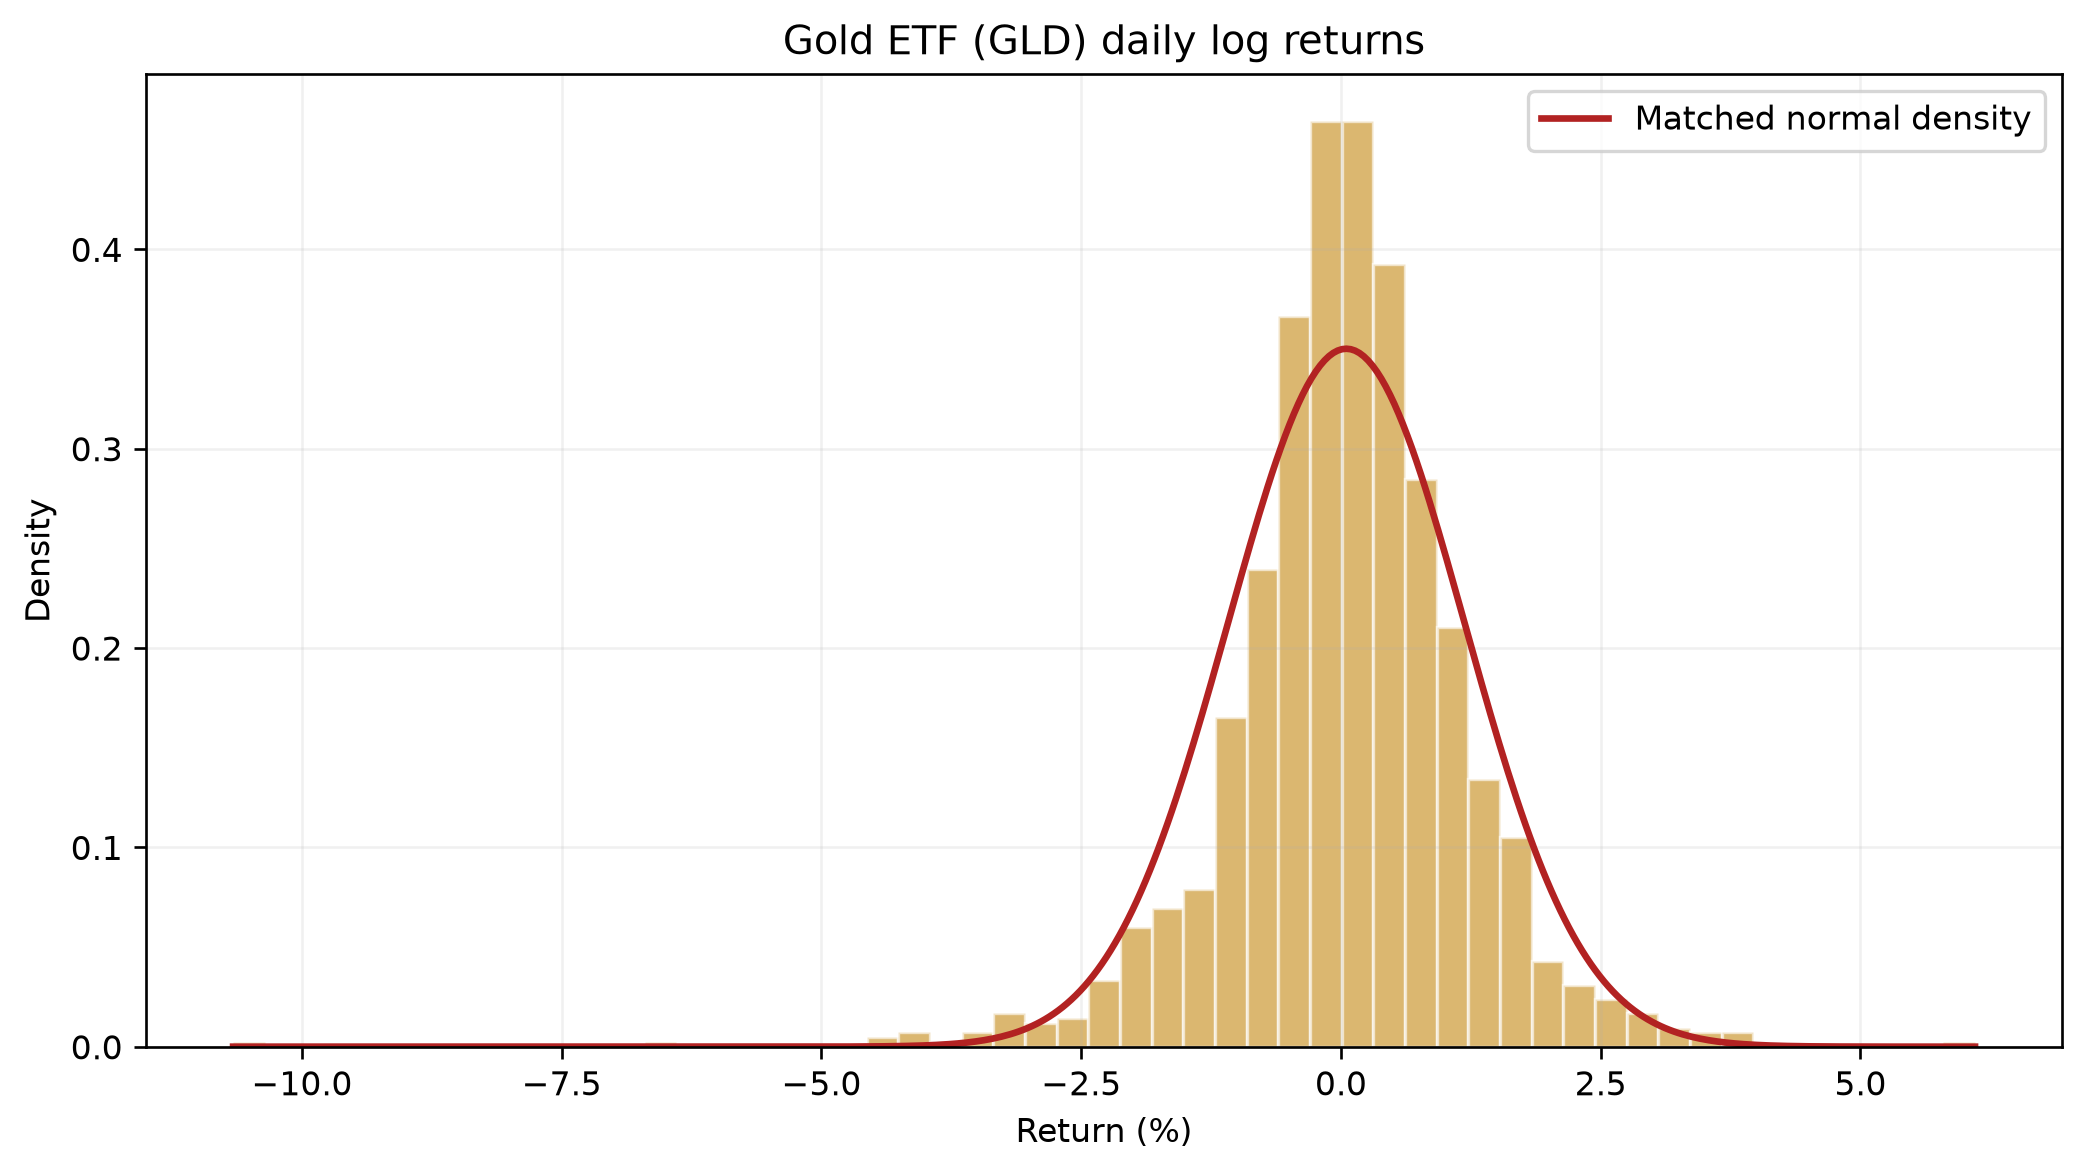
\includegraphics[width=\linewidth]{img/team7_empirical/hist_normal_gold.png}
\end{minipage}\hfill
\begin{minipage}{0.49\textwidth}
\centering
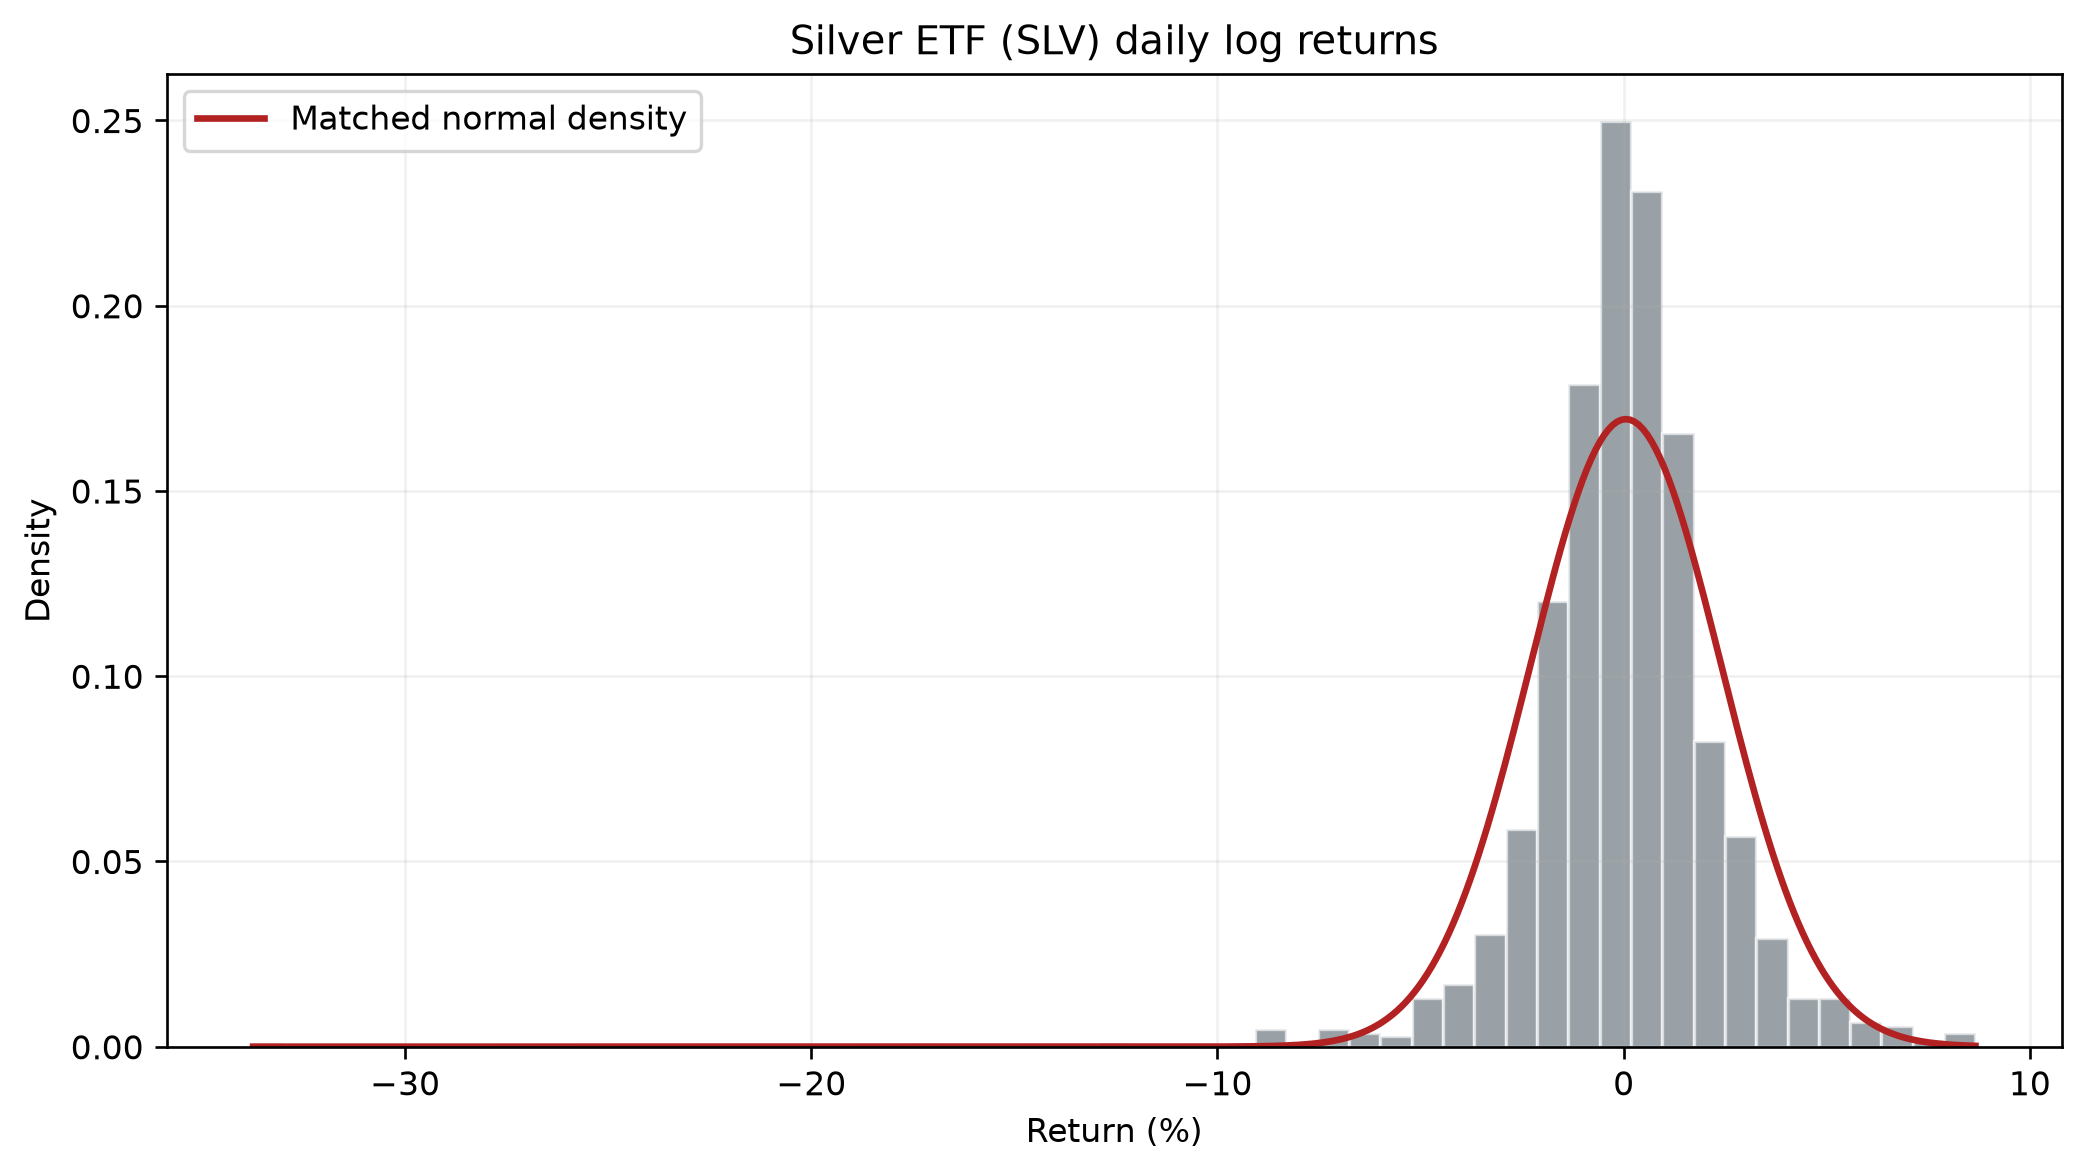
\includegraphics[width=\linewidth]{img/team7_empirical/hist_normal_silver.png}
\end{minipage}
\caption{Current LSE GLD and SLV return histograms with matched normal benchmarks}
\label{fig:t7-return-histograms}
\end{figure}

\begin{figure}[htbp]
\centering
\begin{minipage}{0.49\textwidth}
\centering
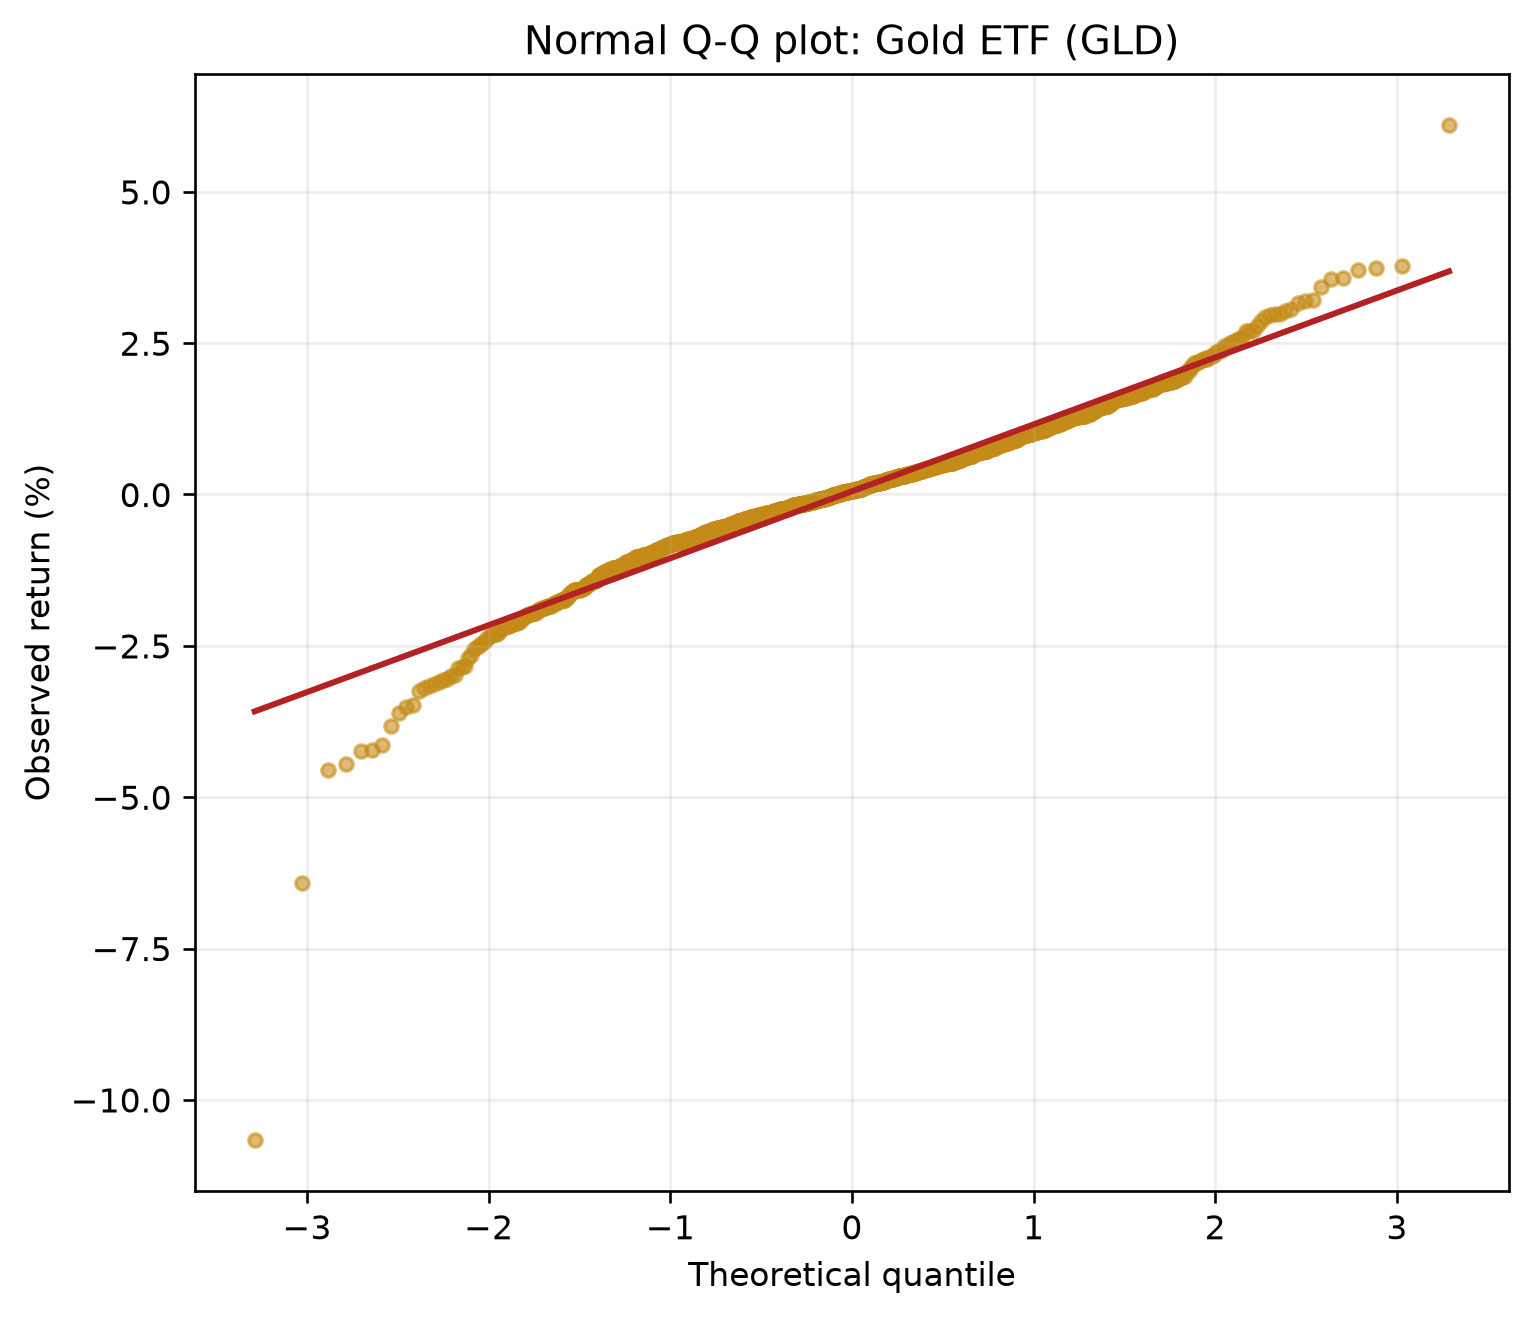
\includegraphics[width=\linewidth]{img/team7_empirical/qqplot_normal_gold.png}
\end{minipage}\hfill
\begin{minipage}{0.49\textwidth}
\centering
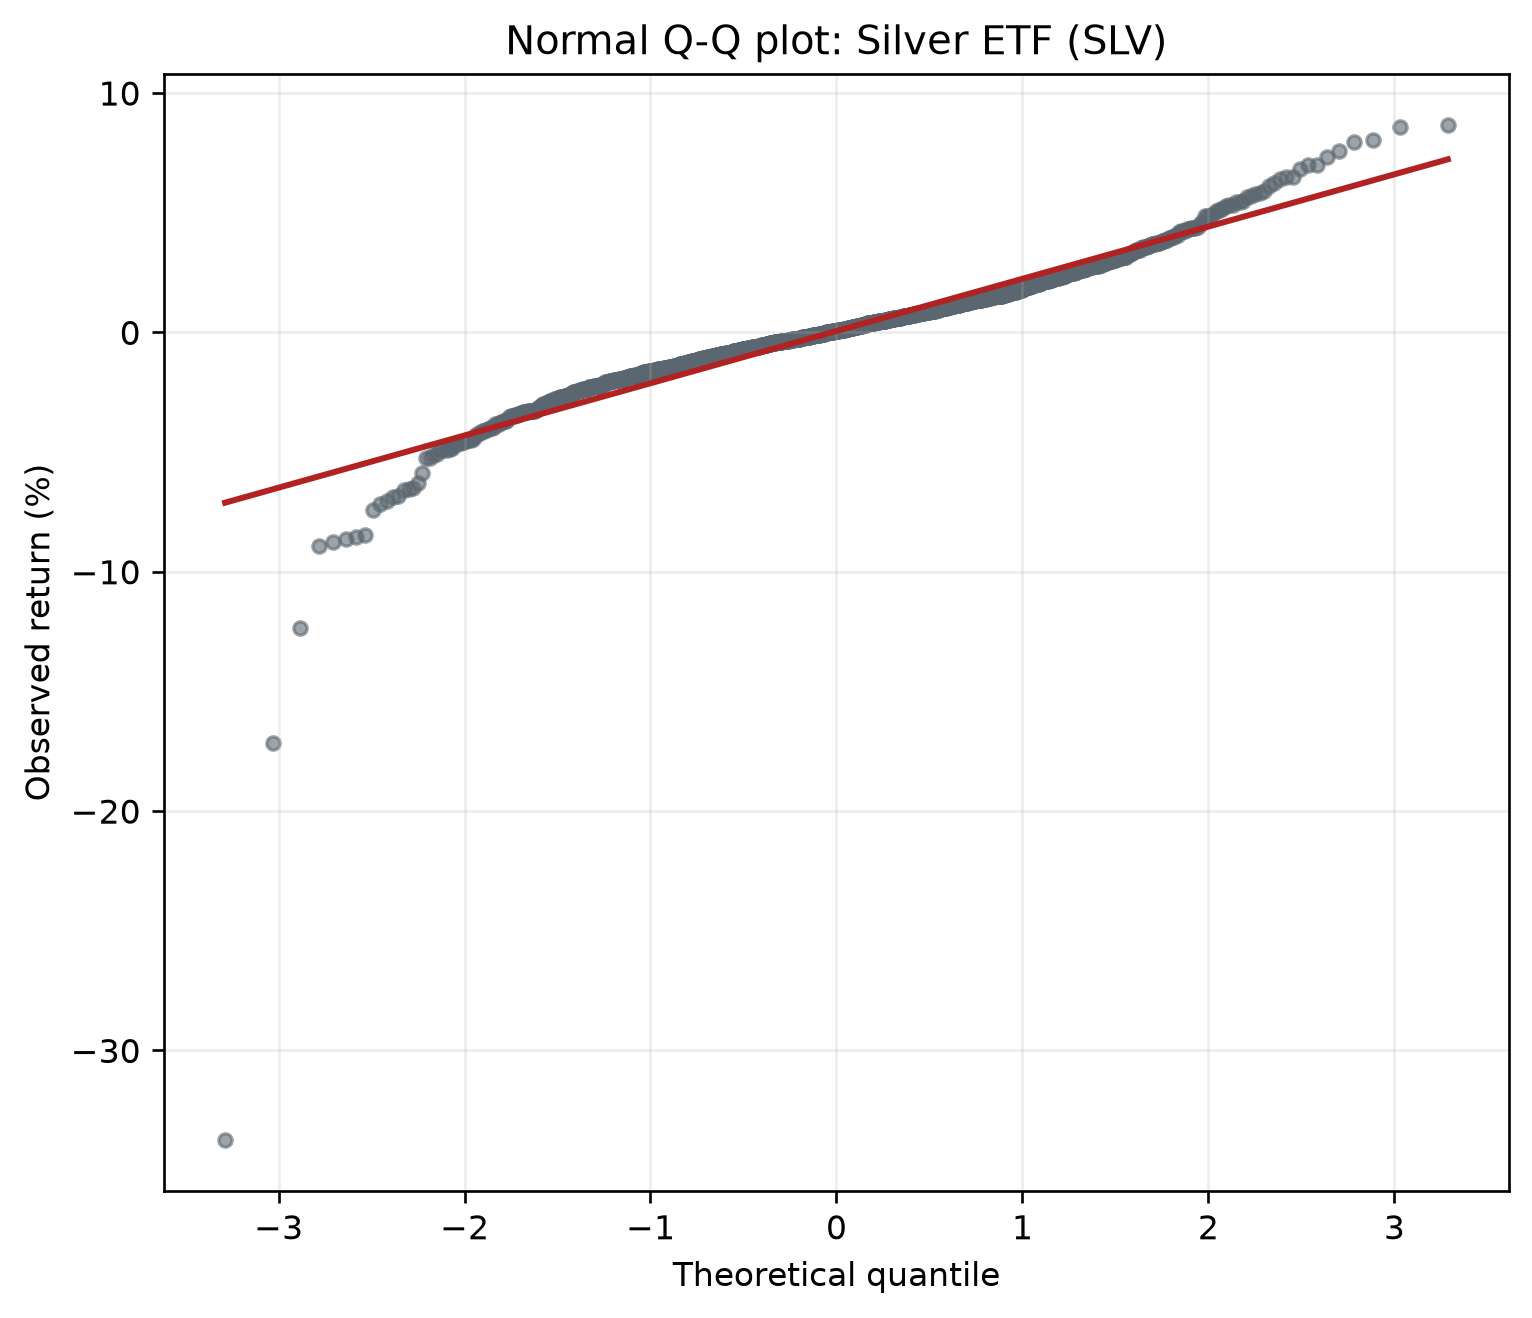
\includegraphics[width=\linewidth]{img/team7_empirical/qqplot_normal_silver.png}
\end{minipage}
\caption{Current LSE normal Q--Q diagnostics for GLD and SLV returns}
\label{fig:t7-return-qqplots}
\end{figure}

Absolute and squared returns show positive serial dependence even when raw
return autocorrelation is weak. Large changes tend to be followed by large
changes of either sign, and shocks decay slowly. This volatility clustering is
the empirical feature that a constant-variance mean model misses most clearly.

\begin{figure}[htbp]
\centering
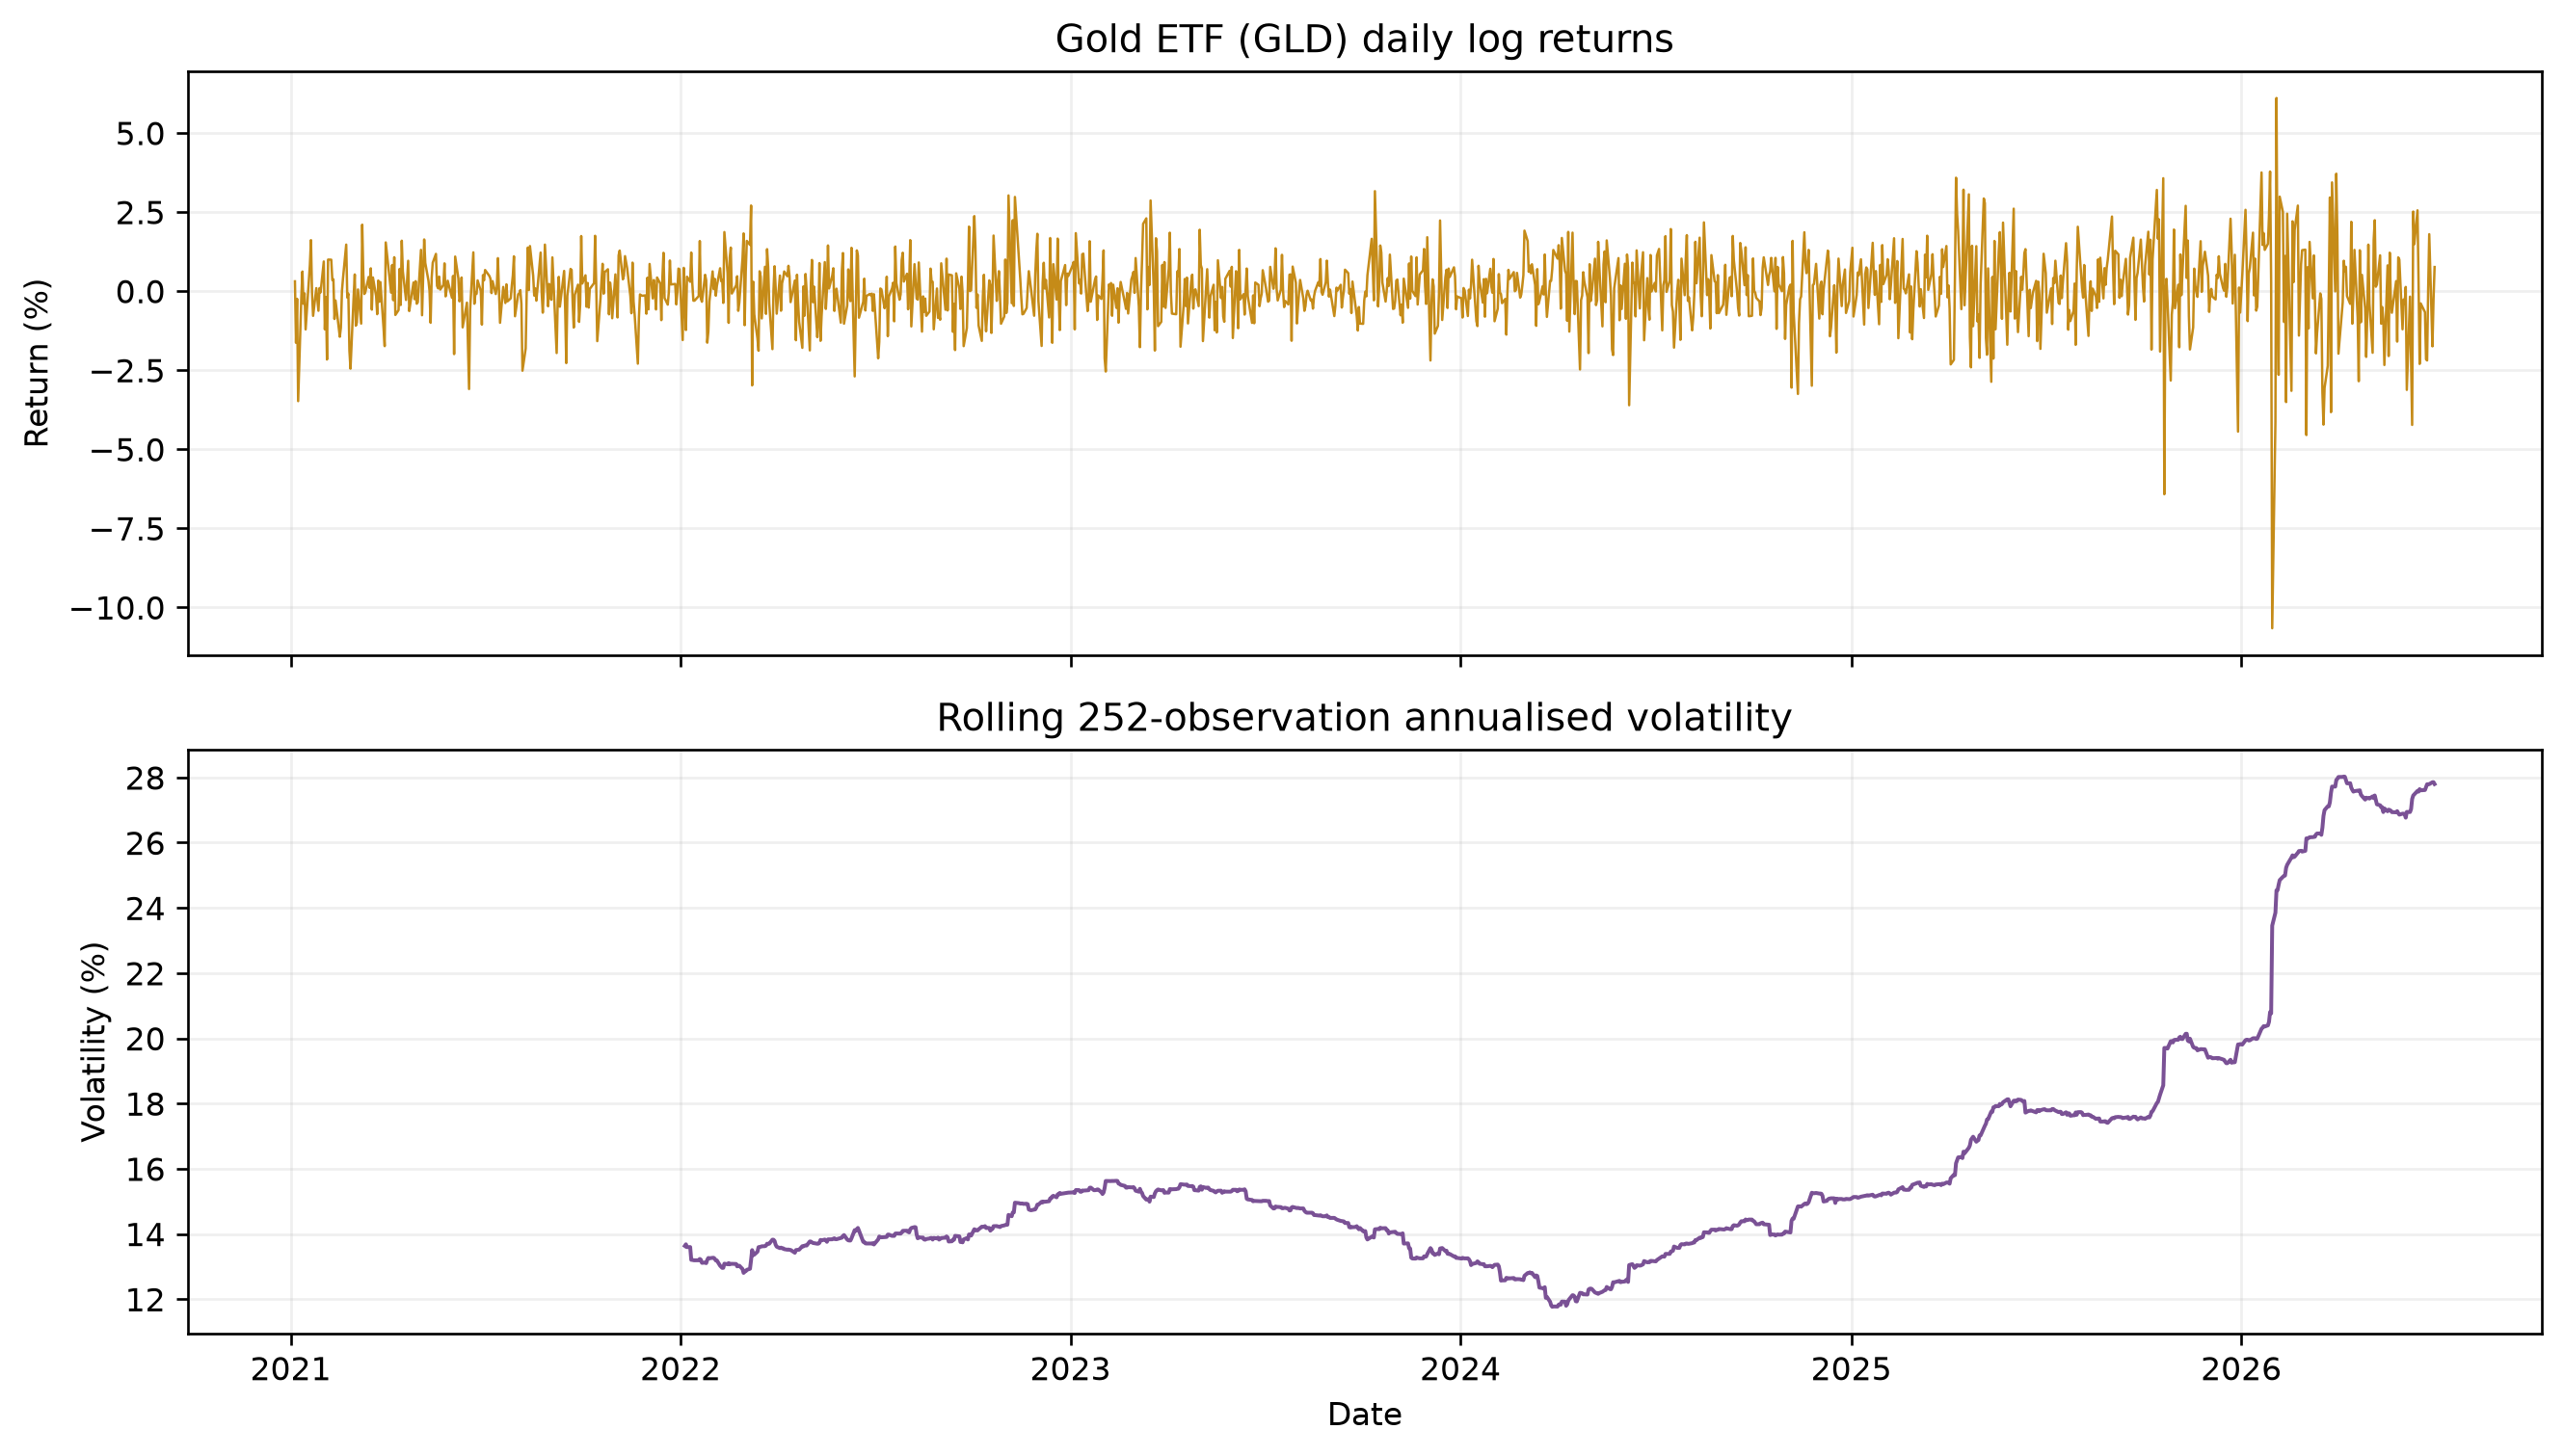
\includegraphics[width=0.88\textwidth]{img/team7_empirical/returns_rollingvol_gold.png}
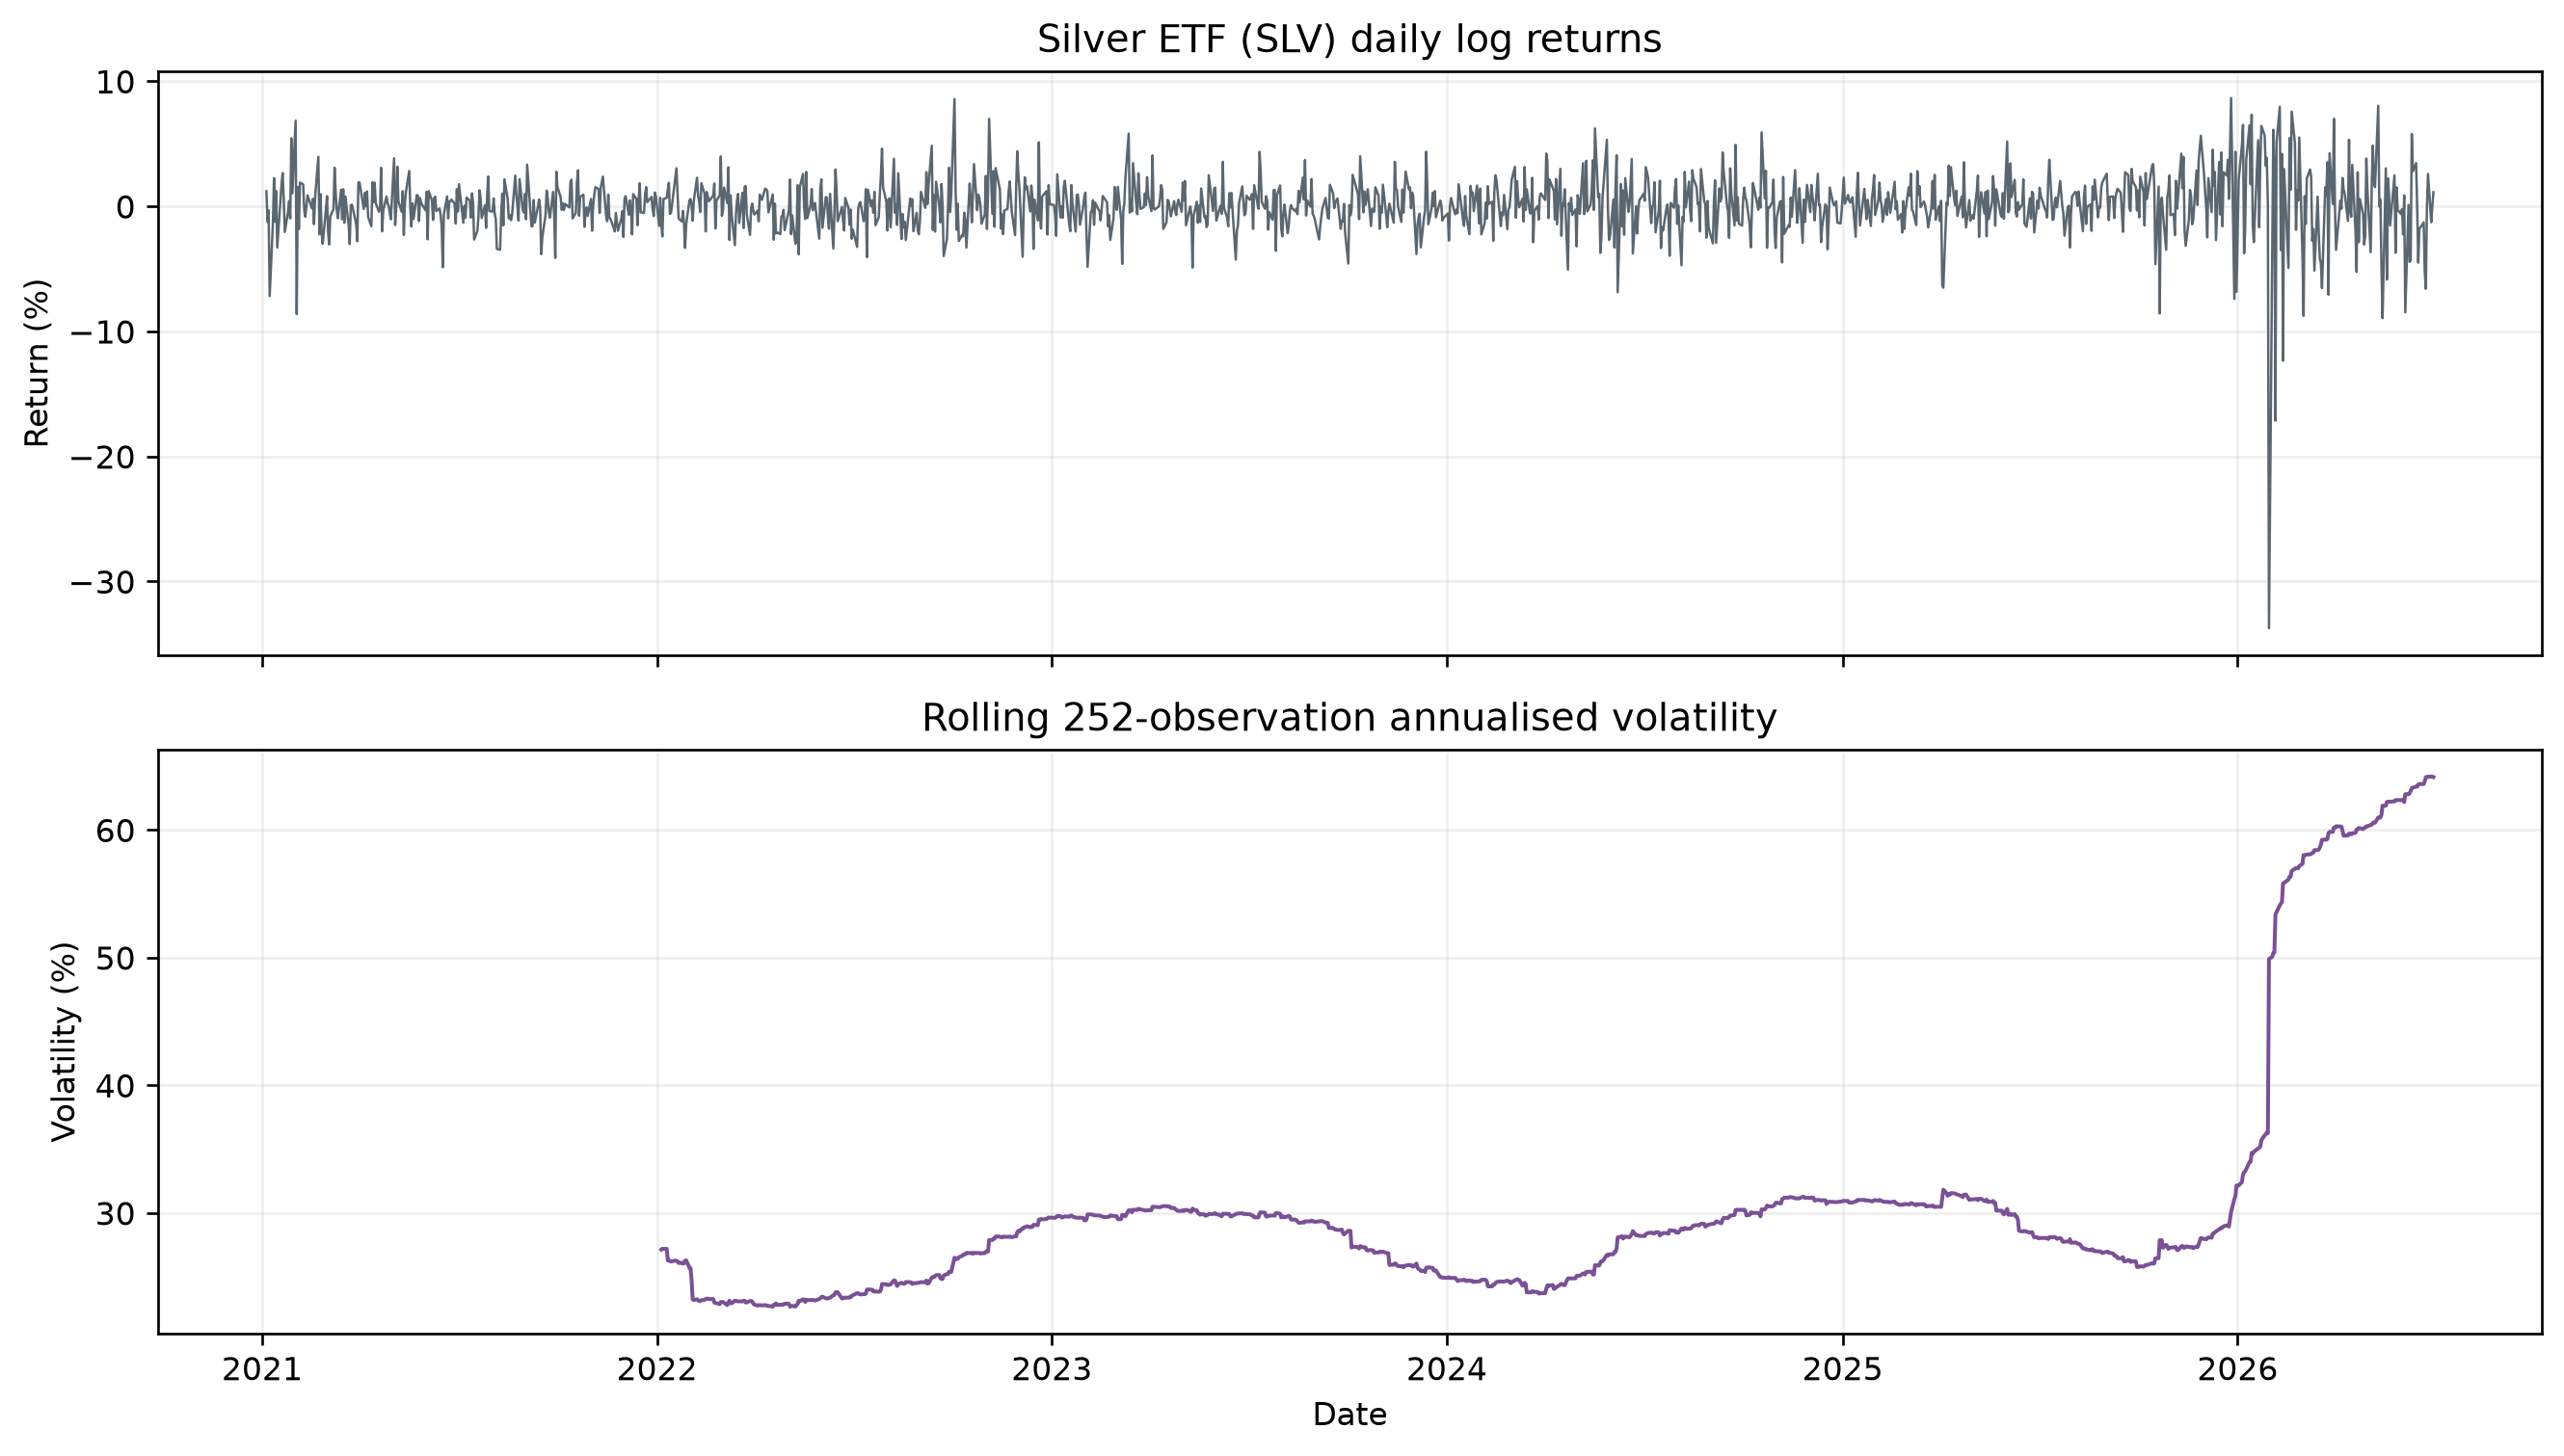
\includegraphics[width=0.88\textwidth]{img/team7_empirical/returns_rollingvol_silver.png}
\caption{Current LSE daily returns and rolling 252-observation annualized volatility for GLD and SLV}
\label{fig:t7-rolling-volatility}
\end{figure}

The ACF panels in Figure~\ref{fig:t7-acf-grid} separate the mean and variance
signals. Raw-return autocorrelations remain close to zero, whereas absolute
and squared returns retain positive dependence over many lags. The compact
persistence statistics in Table~\ref{tab:t7-persistence} reach the same
conclusion.

\begin{figure}[htbp]
\centering
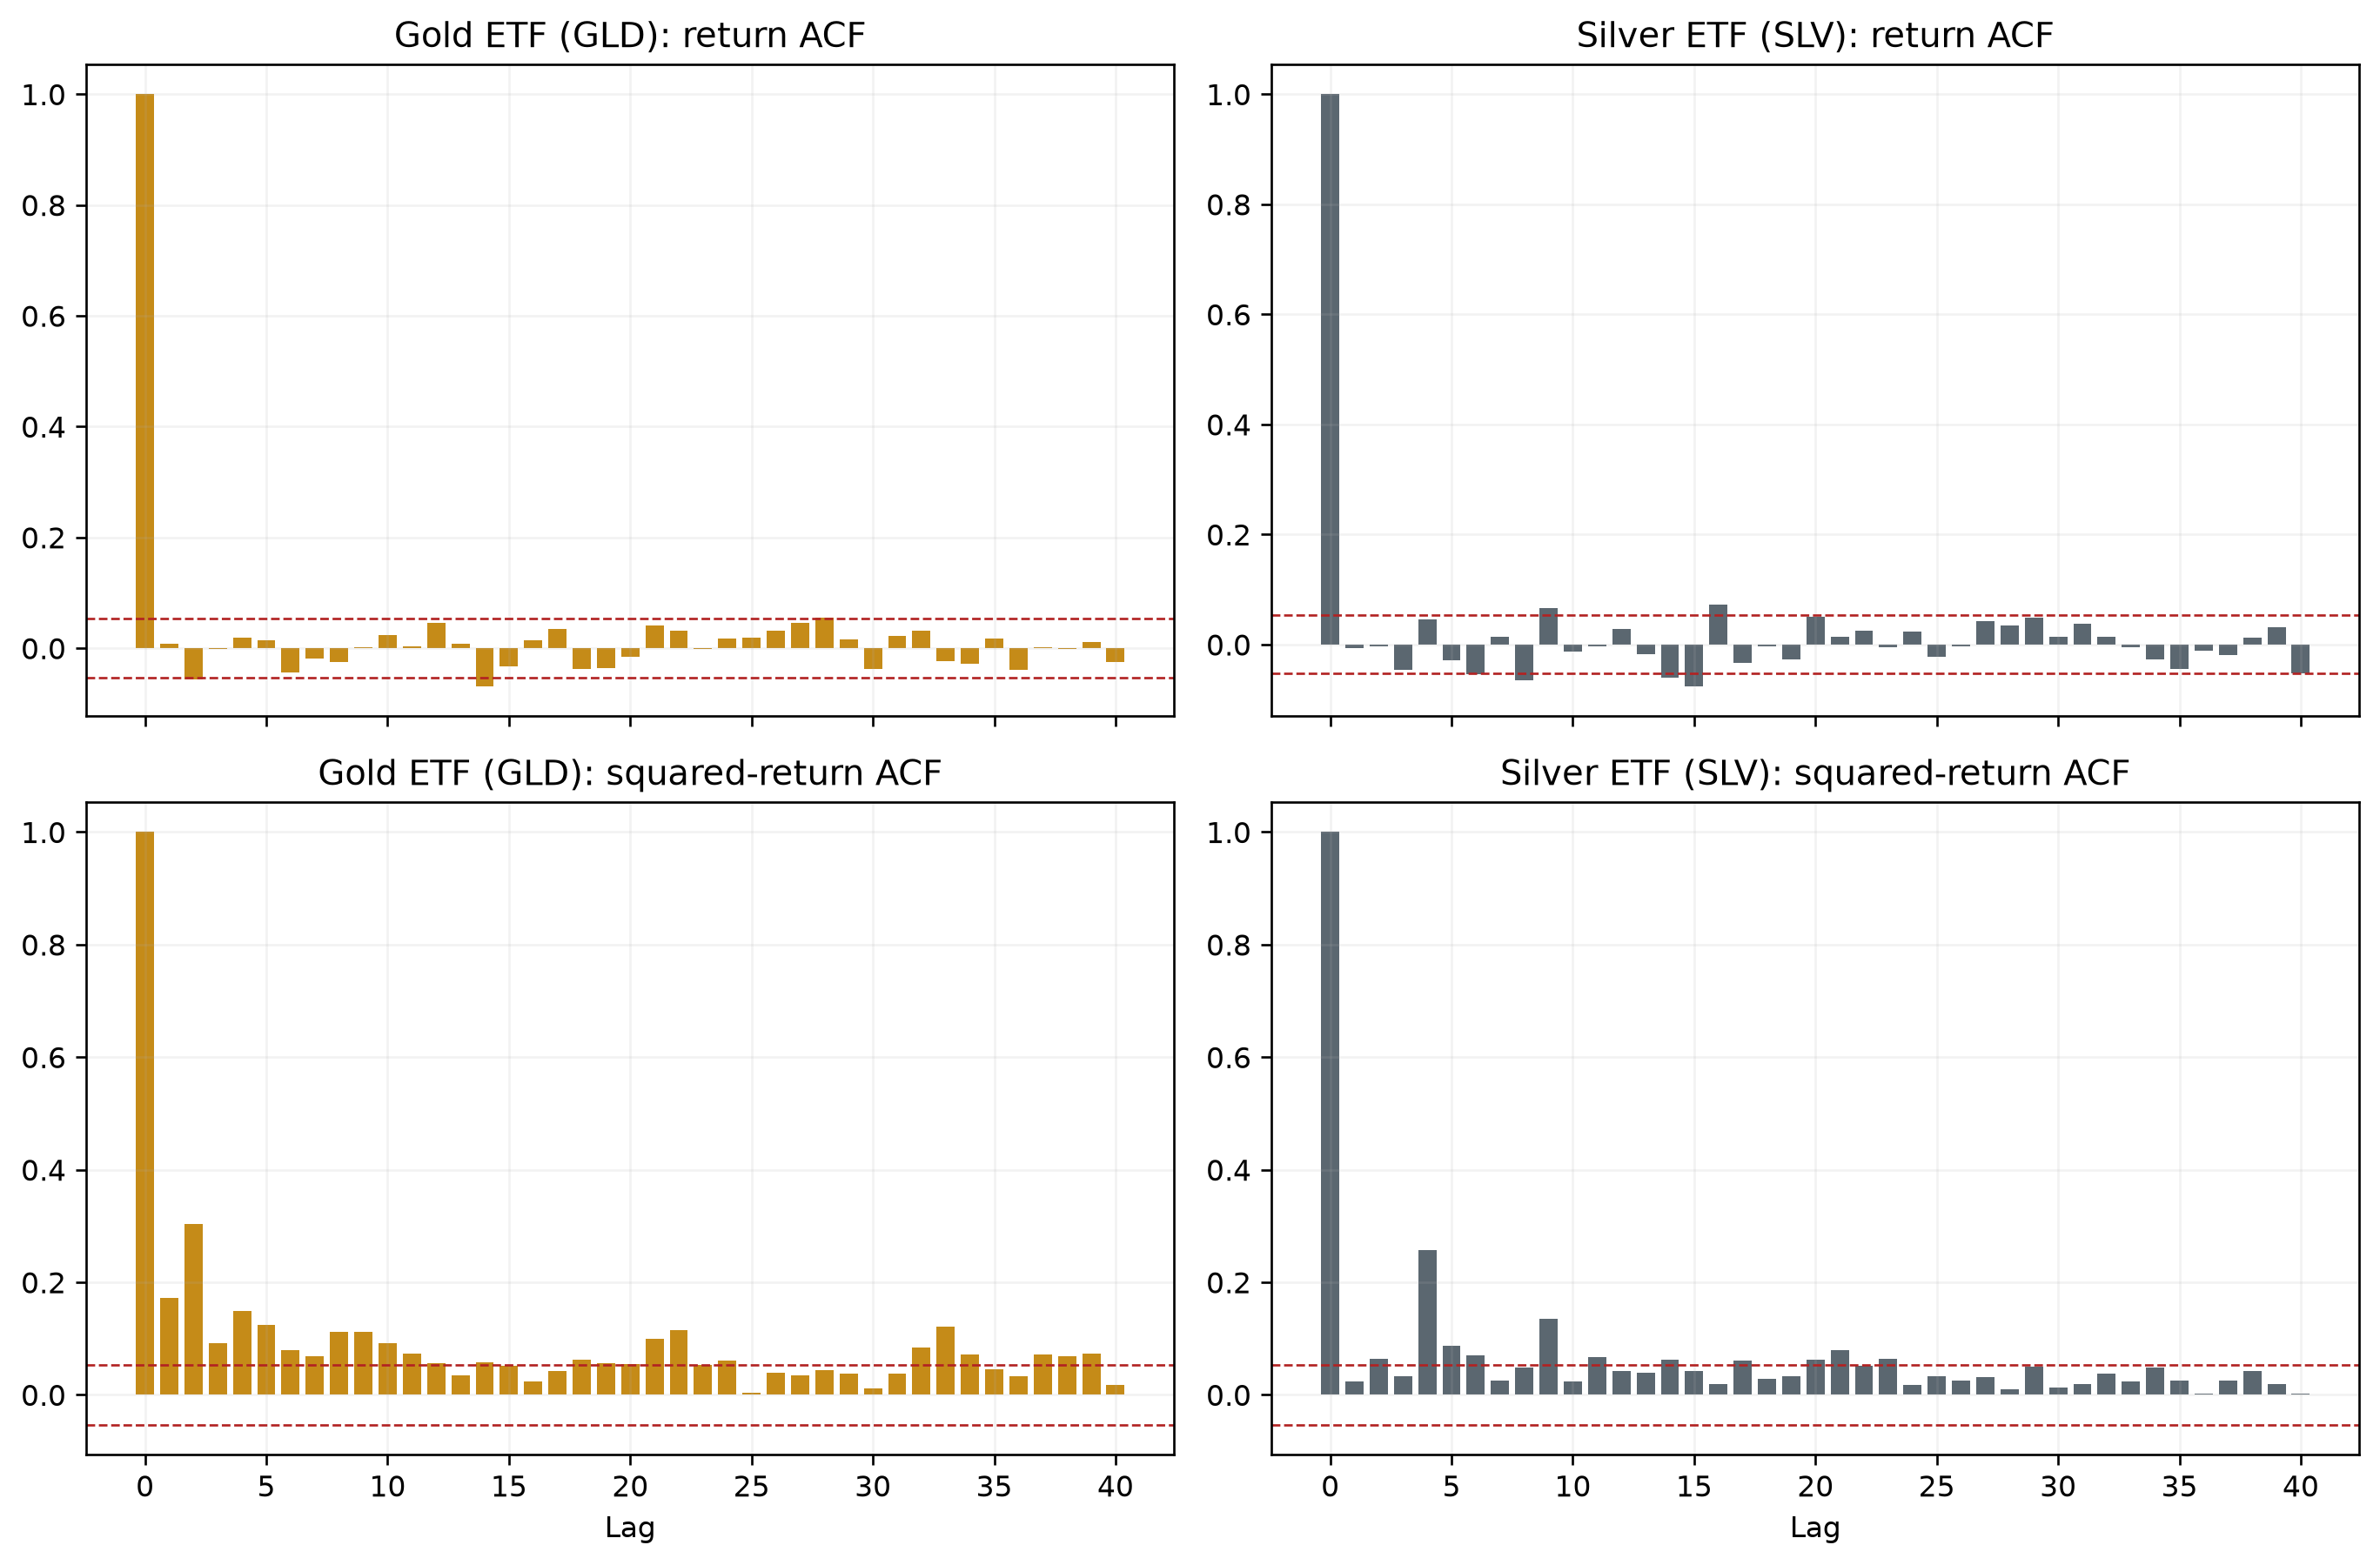
\includegraphics[width=0.95\textwidth]{img/team7_empirical/acf_grid_gold_silver.png}
\caption{Current LSE autocorrelation diagnostics for GLD/SLV returns and squared returns}
\label{fig:t7-acf-grid}
\end{figure}

\begin{table}[htbp]
\centering
\caption{Short-run volatility-persistence diagnostics}
\label{tab:t7-persistence}
\small
\begin{tabular}{lrrr}
\toprule
Asset & $\hat\phi$ & Robust s.e. & $t$-statistic \\
\midrule
Gold   & 0.115 & 0.020 & 5.60 \\
Silver & 0.156 & 0.024 & 6.40 \\
\bottomrule
\end{tabular}
\begin{minipage}{0.94\textwidth}
\footnotesize\emph{Notes:} OLS estimates from
$|r_t|=c+\phi|r_{t-1}|+\varepsilon_t$, with HC1 standard errors. Values
reproduce the compact persistence table in the Team~7 article.
\end{minipage}
\end{table}

\section{ARCH and GARCH Evidence}

An ARCH model makes conditional variance depend on past squared innovations,
while a GARCH model also propagates its own lagged variance. For the benchmark
GARCH$(1,1)$,
\[
 r_t=\mu+\varepsilon_t,\qquad
 \sigma_t^2=\omega+\alpha\varepsilon_{t-1}^2+\beta\sigma_{t-1}^2.
\]
The unified branch fits a Gaussian GARCH$(1,1)$ directly to the current LSE
returns. The estimates are
$(\hat\omega,\hat\alpha,\hat\beta)\approx(0.05385,0.10894,0.84798)$ for GLD and
$(0.04080,0.05453,0.93900)$ for SLV when returns are expressed in percentage
points. Both optimizers converge and $\hat\alpha+\hat\beta<1$; persistence is
especially high for SLV.

\begin{table}[htbp]
\centering
\caption{GARCH(1,1) estimates for gold and silver daily returns}
\label{tab:t7-garch-parameters}
\small
\resizebox{0.96\textwidth}{!}{%
\begin{tabular}{lrrrrrr}
\toprule
Asset & $\hat\mu$ & $\hat\omega$ & $\hat\alpha$ & $\hat\beta$
& $\hat\alpha+\hat\beta$ & $\hat\sigma^2_{\infty}$ \\
\midrule
GLD & 0.03494 & 0.05385 & 0.10894 & 0.84798 & 0.95692 & 1.2500 \\
SLV & 0.01495 & 0.04080 & 0.05453 & 0.93900 & 0.99353 & 6.3067 \\
\bottomrule
\end{tabular}}
\begin{minipage}{0.94\textwidth}
\footnotesize\emph{Notes:} Returns and conditional volatilities are expressed
in percentage units. When $\hat\alpha+\hat\beta<1$,
$\hat\sigma^2_{\infty}=\hat\omega/(1-\hat\alpha-\hat\beta)$.
\end{minipage}
\end{table}

Figure~\ref{fig:t7-garch-conditional-volatility} shows the regenerated fitted
conditional-volatility paths. Silver fluctuates around a higher baseline and
has larger spikes; for both metals the decay after stress episodes is gradual,
as implied by the near-unit persistence estimates.

\begin{figure}[htbp]
\centering
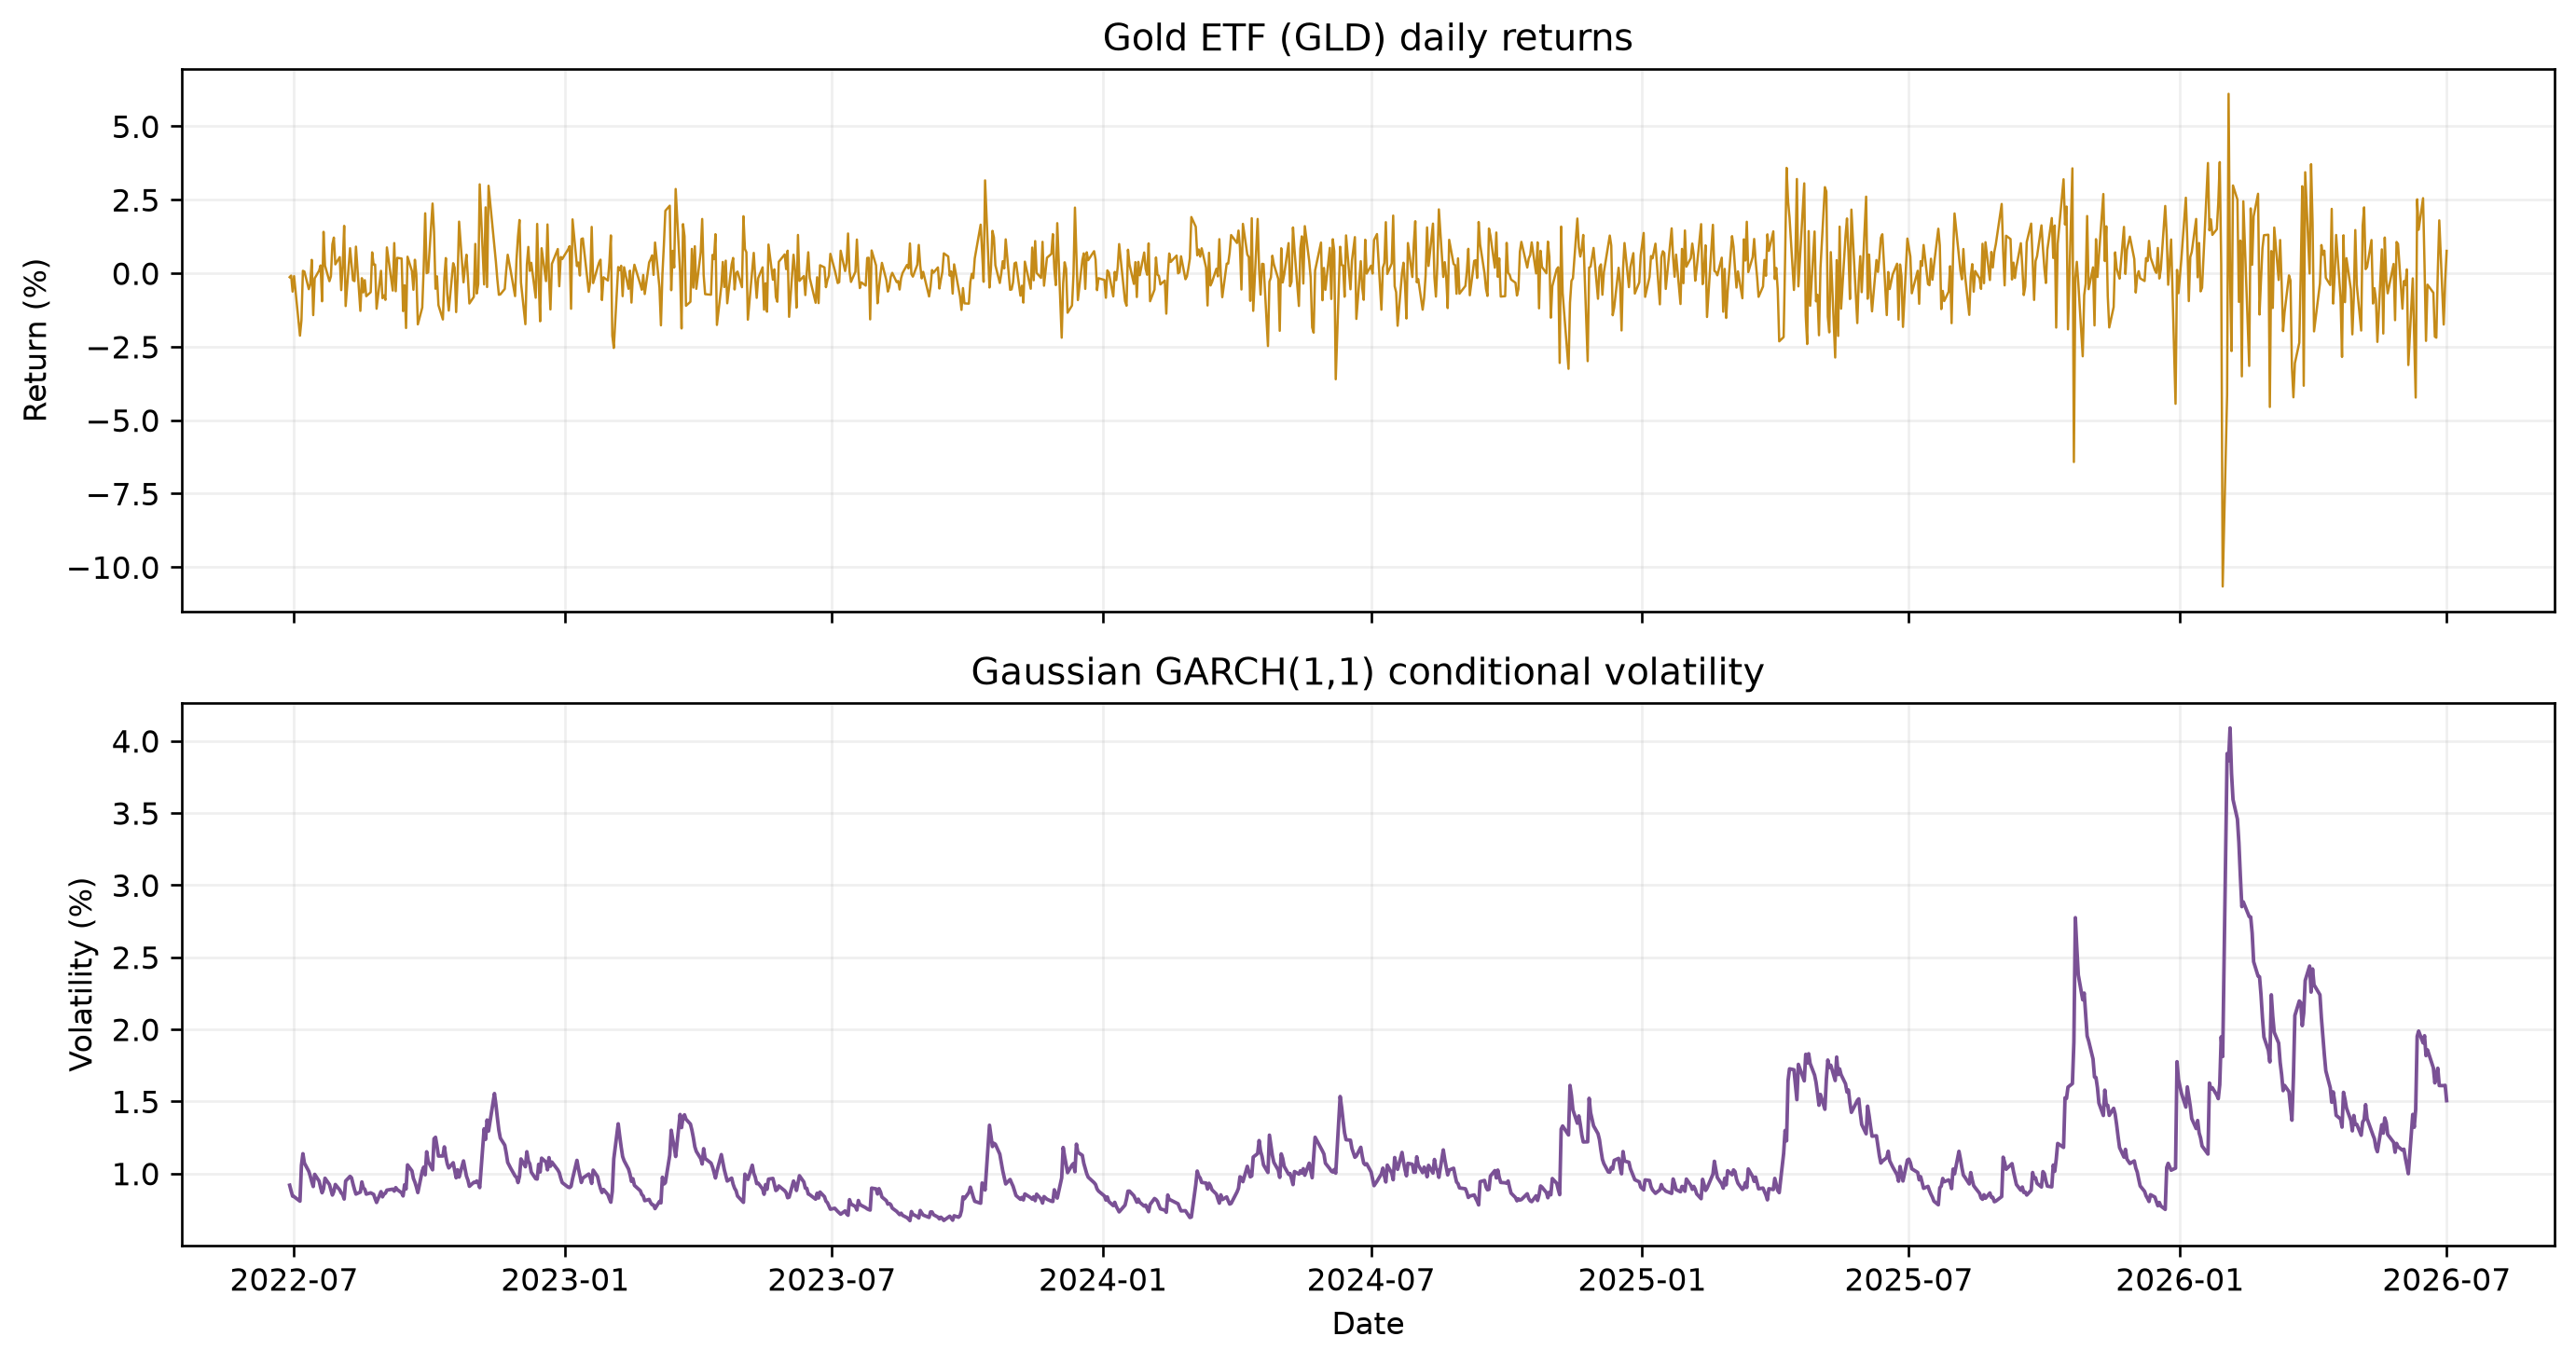
\includegraphics[width=0.90\textwidth]{img/team7_empirical/garch_condvol_gold.png}
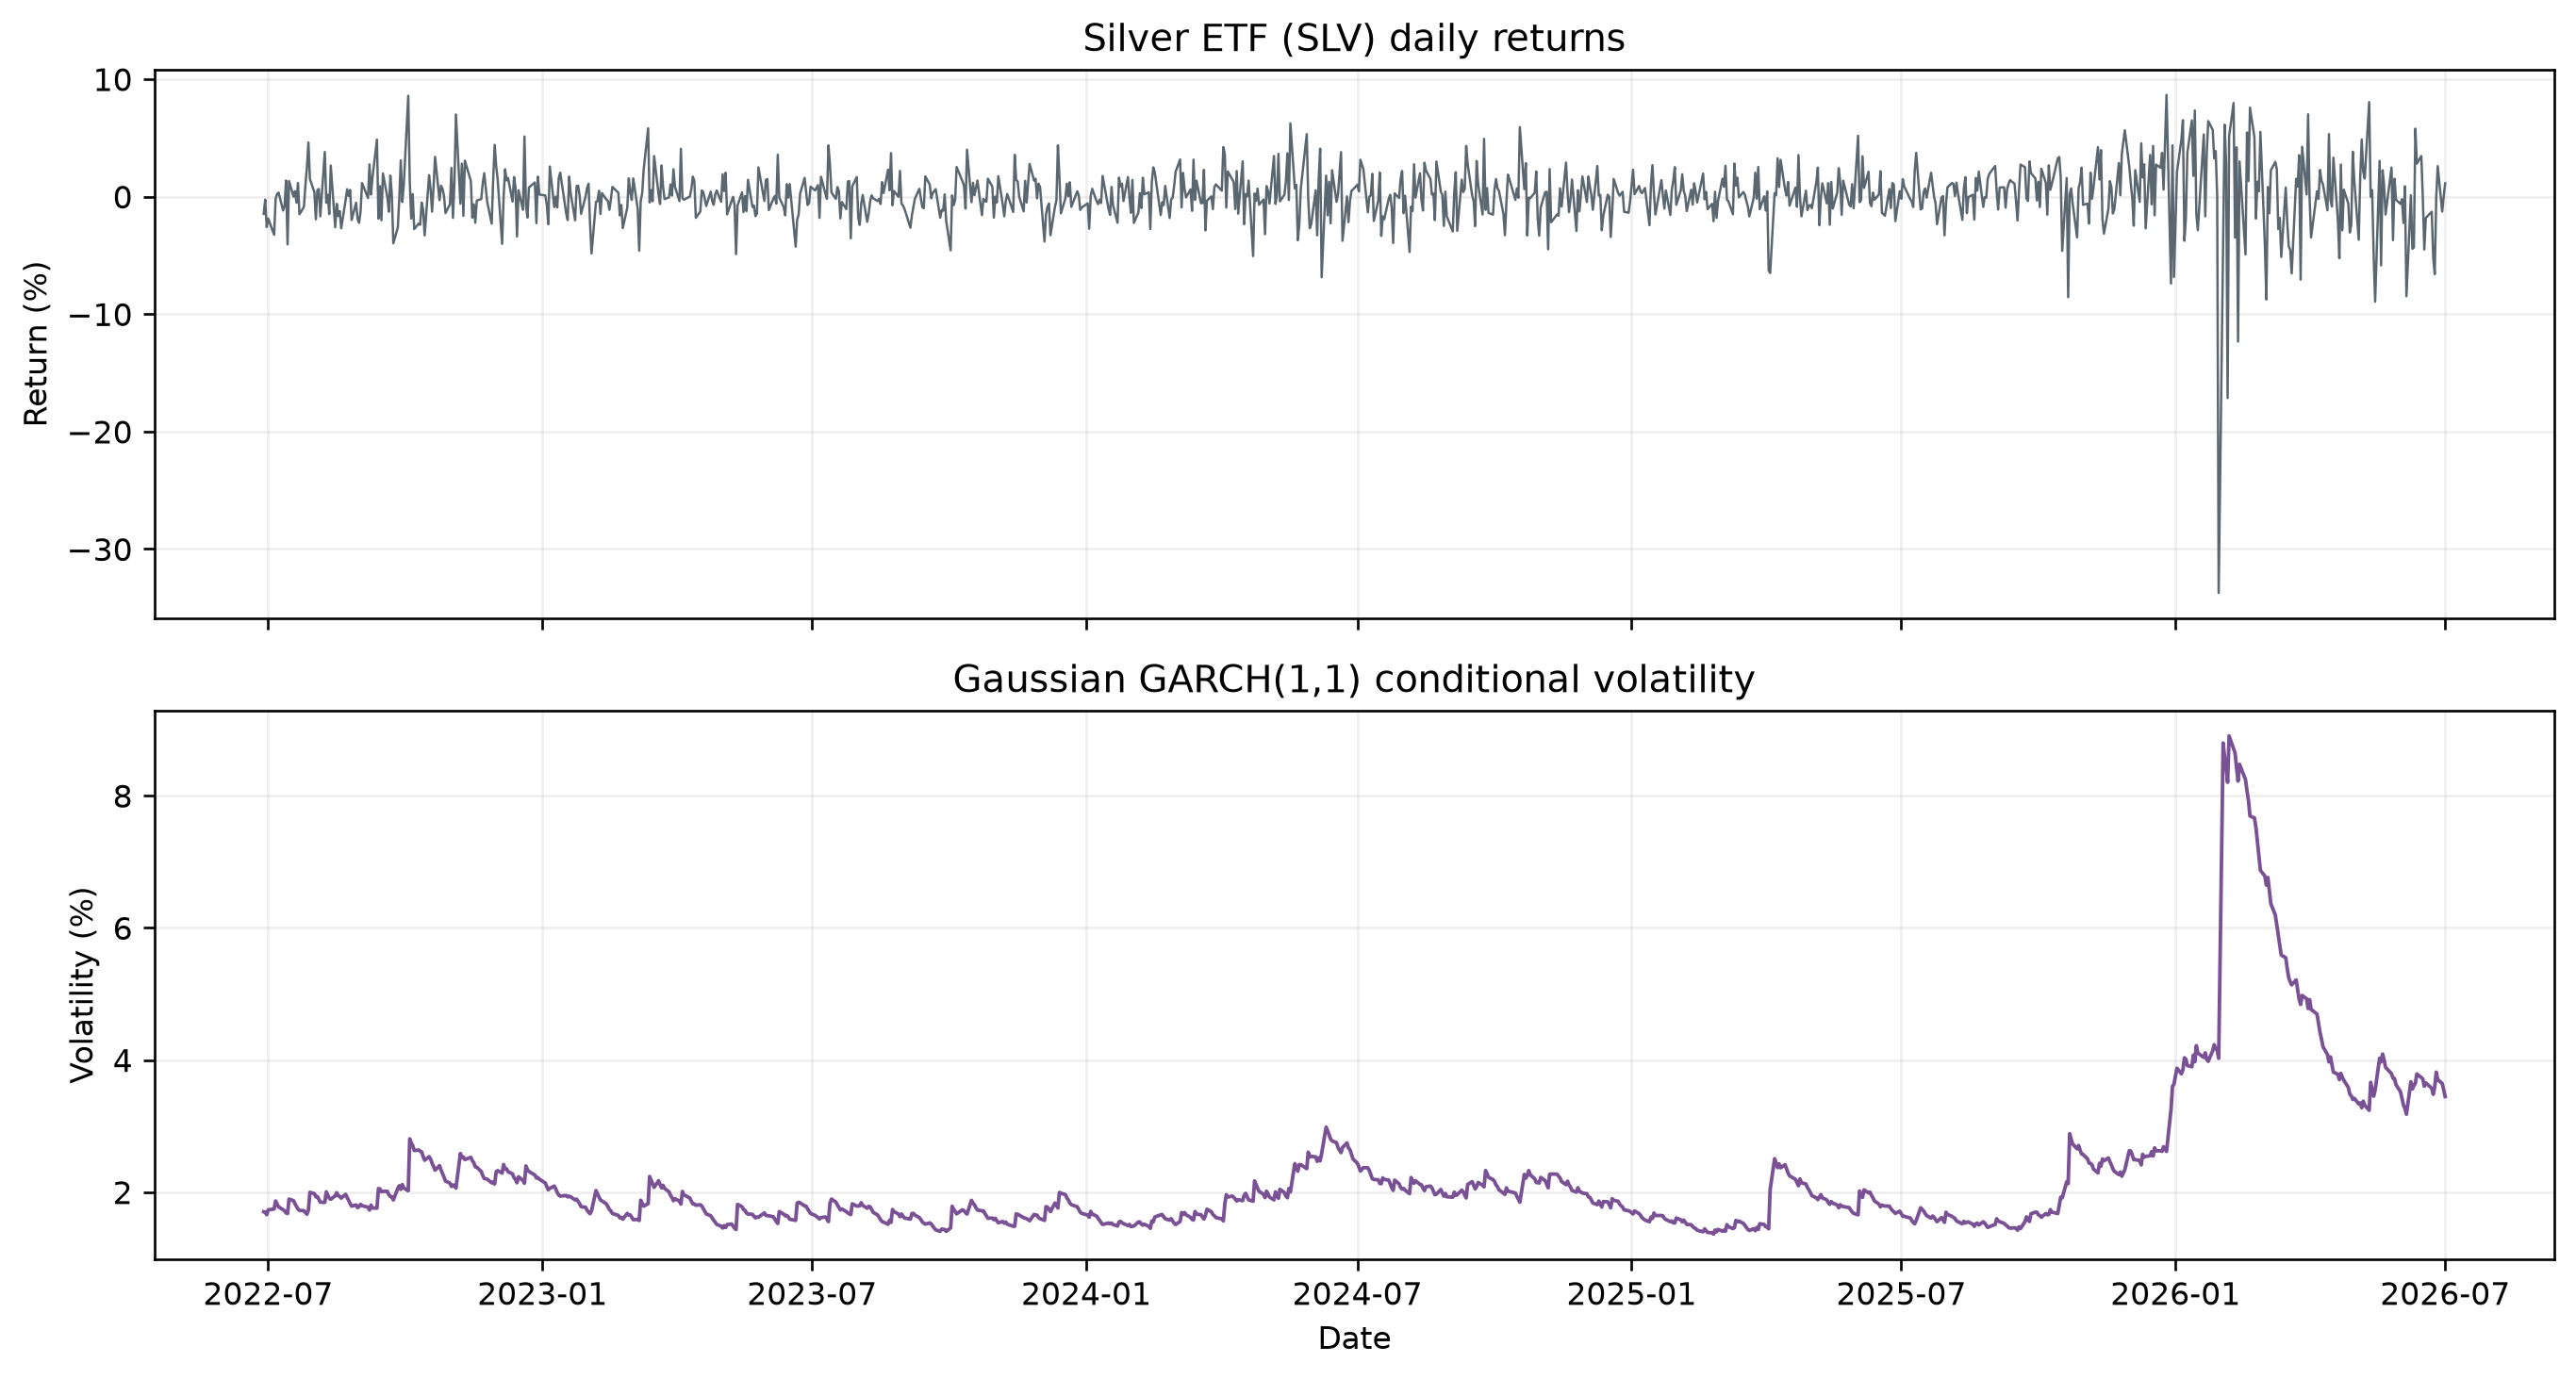
\includegraphics[width=0.90\textwidth]{img/team7_empirical/garch_condvol_silver.png}
\caption{Current LSE Gaussian GARCH(1,1) conditional volatility for GLD and SLV}
\label{fig:t7-garch-conditional-volatility}
\end{figure}

For historical comparison, the frozen Team~7 end-of-sample variance forecasts in
Table~\ref{tab:t7-garch-forecasts} show the same slow mean reversion. In that legacy run, gold
moves from approximately $0.981$ to $1.002$ squared percentage points over ten
days, toward a long-run level of $1.211$; silver moves from $2.686$ to $2.791$,
toward $4.235$.

\begin{table}[htbp]
\centering
\caption{Frozen Team~7 end-of-sample GARCH conditional-variance forecasts}
\label{tab:t7-garch-forecasts}
\small
\begin{tabular}{crr@{\qquad}crr}
\toprule
$h$ & Gold & Silver & $h$ & Gold & Silver \\
\midrule
1 & 0.981250 & 2.685694 &  6 & 0.993096 & 2.745300 \\
2 & 0.983669 & 2.697803 &  7 & 0.995391 & 2.756943 \\
3 & 0.986064 & 2.709817 &  8 & 0.997662 & 2.768495 \\
4 & 0.988433 & 2.721737 &  9 & 0.999908 & 2.779957 \\
5 & 0.990777 & 2.733565 & 10 & 1.002131 & 2.791329 \\
\bottomrule
\end{tabular}
\begin{minipage}{0.90\textwidth}
\footnotesize\emph{Notes:} Forecast horizon $h$ is measured in trading days;
variances are in squared percentage-return units.
\end{minipage}
\end{table}

These estimates show why GARCH is useful: it converts clustering into a
dynamic conditional-variance forecast. GARCH remains a discrete-time model,
and this is a strength for empirical diagnosis rather than a conceptual flaw.
Its role here is to show that the relevant predictable object is volatility
more than the daily conditional mean.

\section{Long-Memory Cross-Check: GPH and Fractional Differencing}

GARCH captures short-run clustering with a recursive conditional variance. A
separate question is whether a volatility proxy also displays hyperbolically
decaying, long-range dependence. Team~7 applied the semiparametric
Geweke--Porter--Hudak estimator to absolute daily returns. The frozen published
estimates in Table~\ref{tab:t7-gph} are positive and precisely estimated. The
current LSE figure rebuild estimates $d=0.452$ for GLD and clips the SLV
estimate at the implementation boundary $d=0.490$; it does not reuse the
published point estimates.

\begin{table}[htbp]
\centering
\caption{Frozen Team~7 GPH estimates of the fractional differencing parameter for absolute returns}
\label{tab:t7-gph}
\small
\begin{tabular}{lrrr}
\toprule
Asset & $\hat d$ & s.e.($\hat d$) & $t$-statistic \\
\midrule
Gold   & 0.576 & 0.090 & 6.39 \\
Silver & 0.552 & 0.080 & 6.91 \\
\bottomrule
\end{tabular}
\end{table}

The regenerated visual evidence is consistent with persistent absolute returns. Their
autocorrelations remain positive across many lags in
Figure~\ref{fig:t7-absolute-return-acf}, while fractional filtering visibly
reduces low-frequency persistence in
Figure~\ref{fig:t7-fractional-differencing}.

\begin{figure}[htbp]
\centering
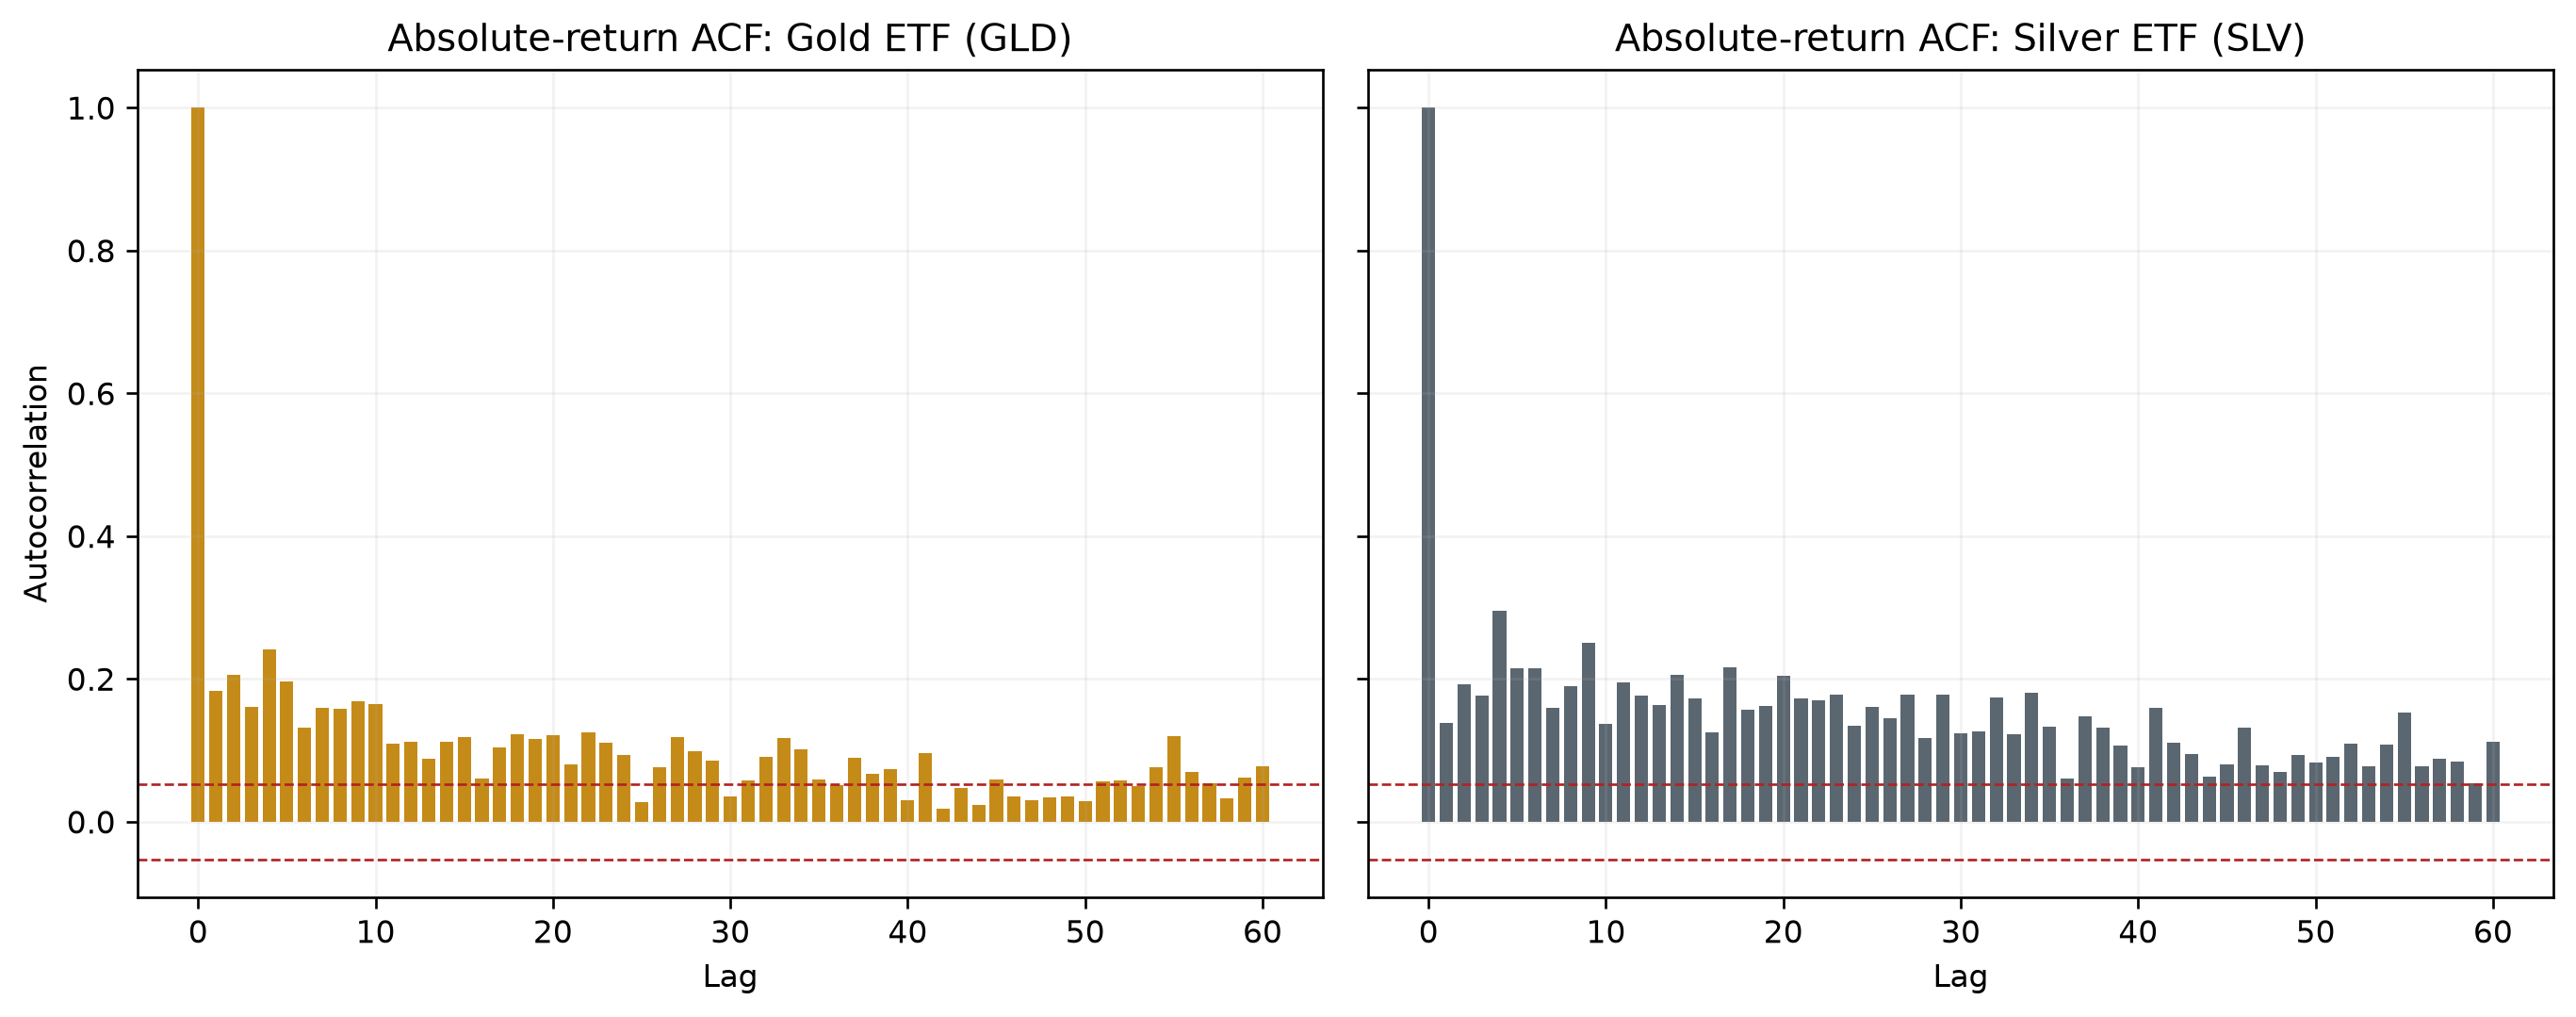
\includegraphics[width=0.88\textwidth]{img/team7_empirical/acf_abs_returns_gold_silver.png}
\caption{Current LSE autocorrelation functions of GLD and SLV absolute returns}
\label{fig:t7-absolute-return-acf}
\end{figure}

\begin{figure}[htbp]
\centering
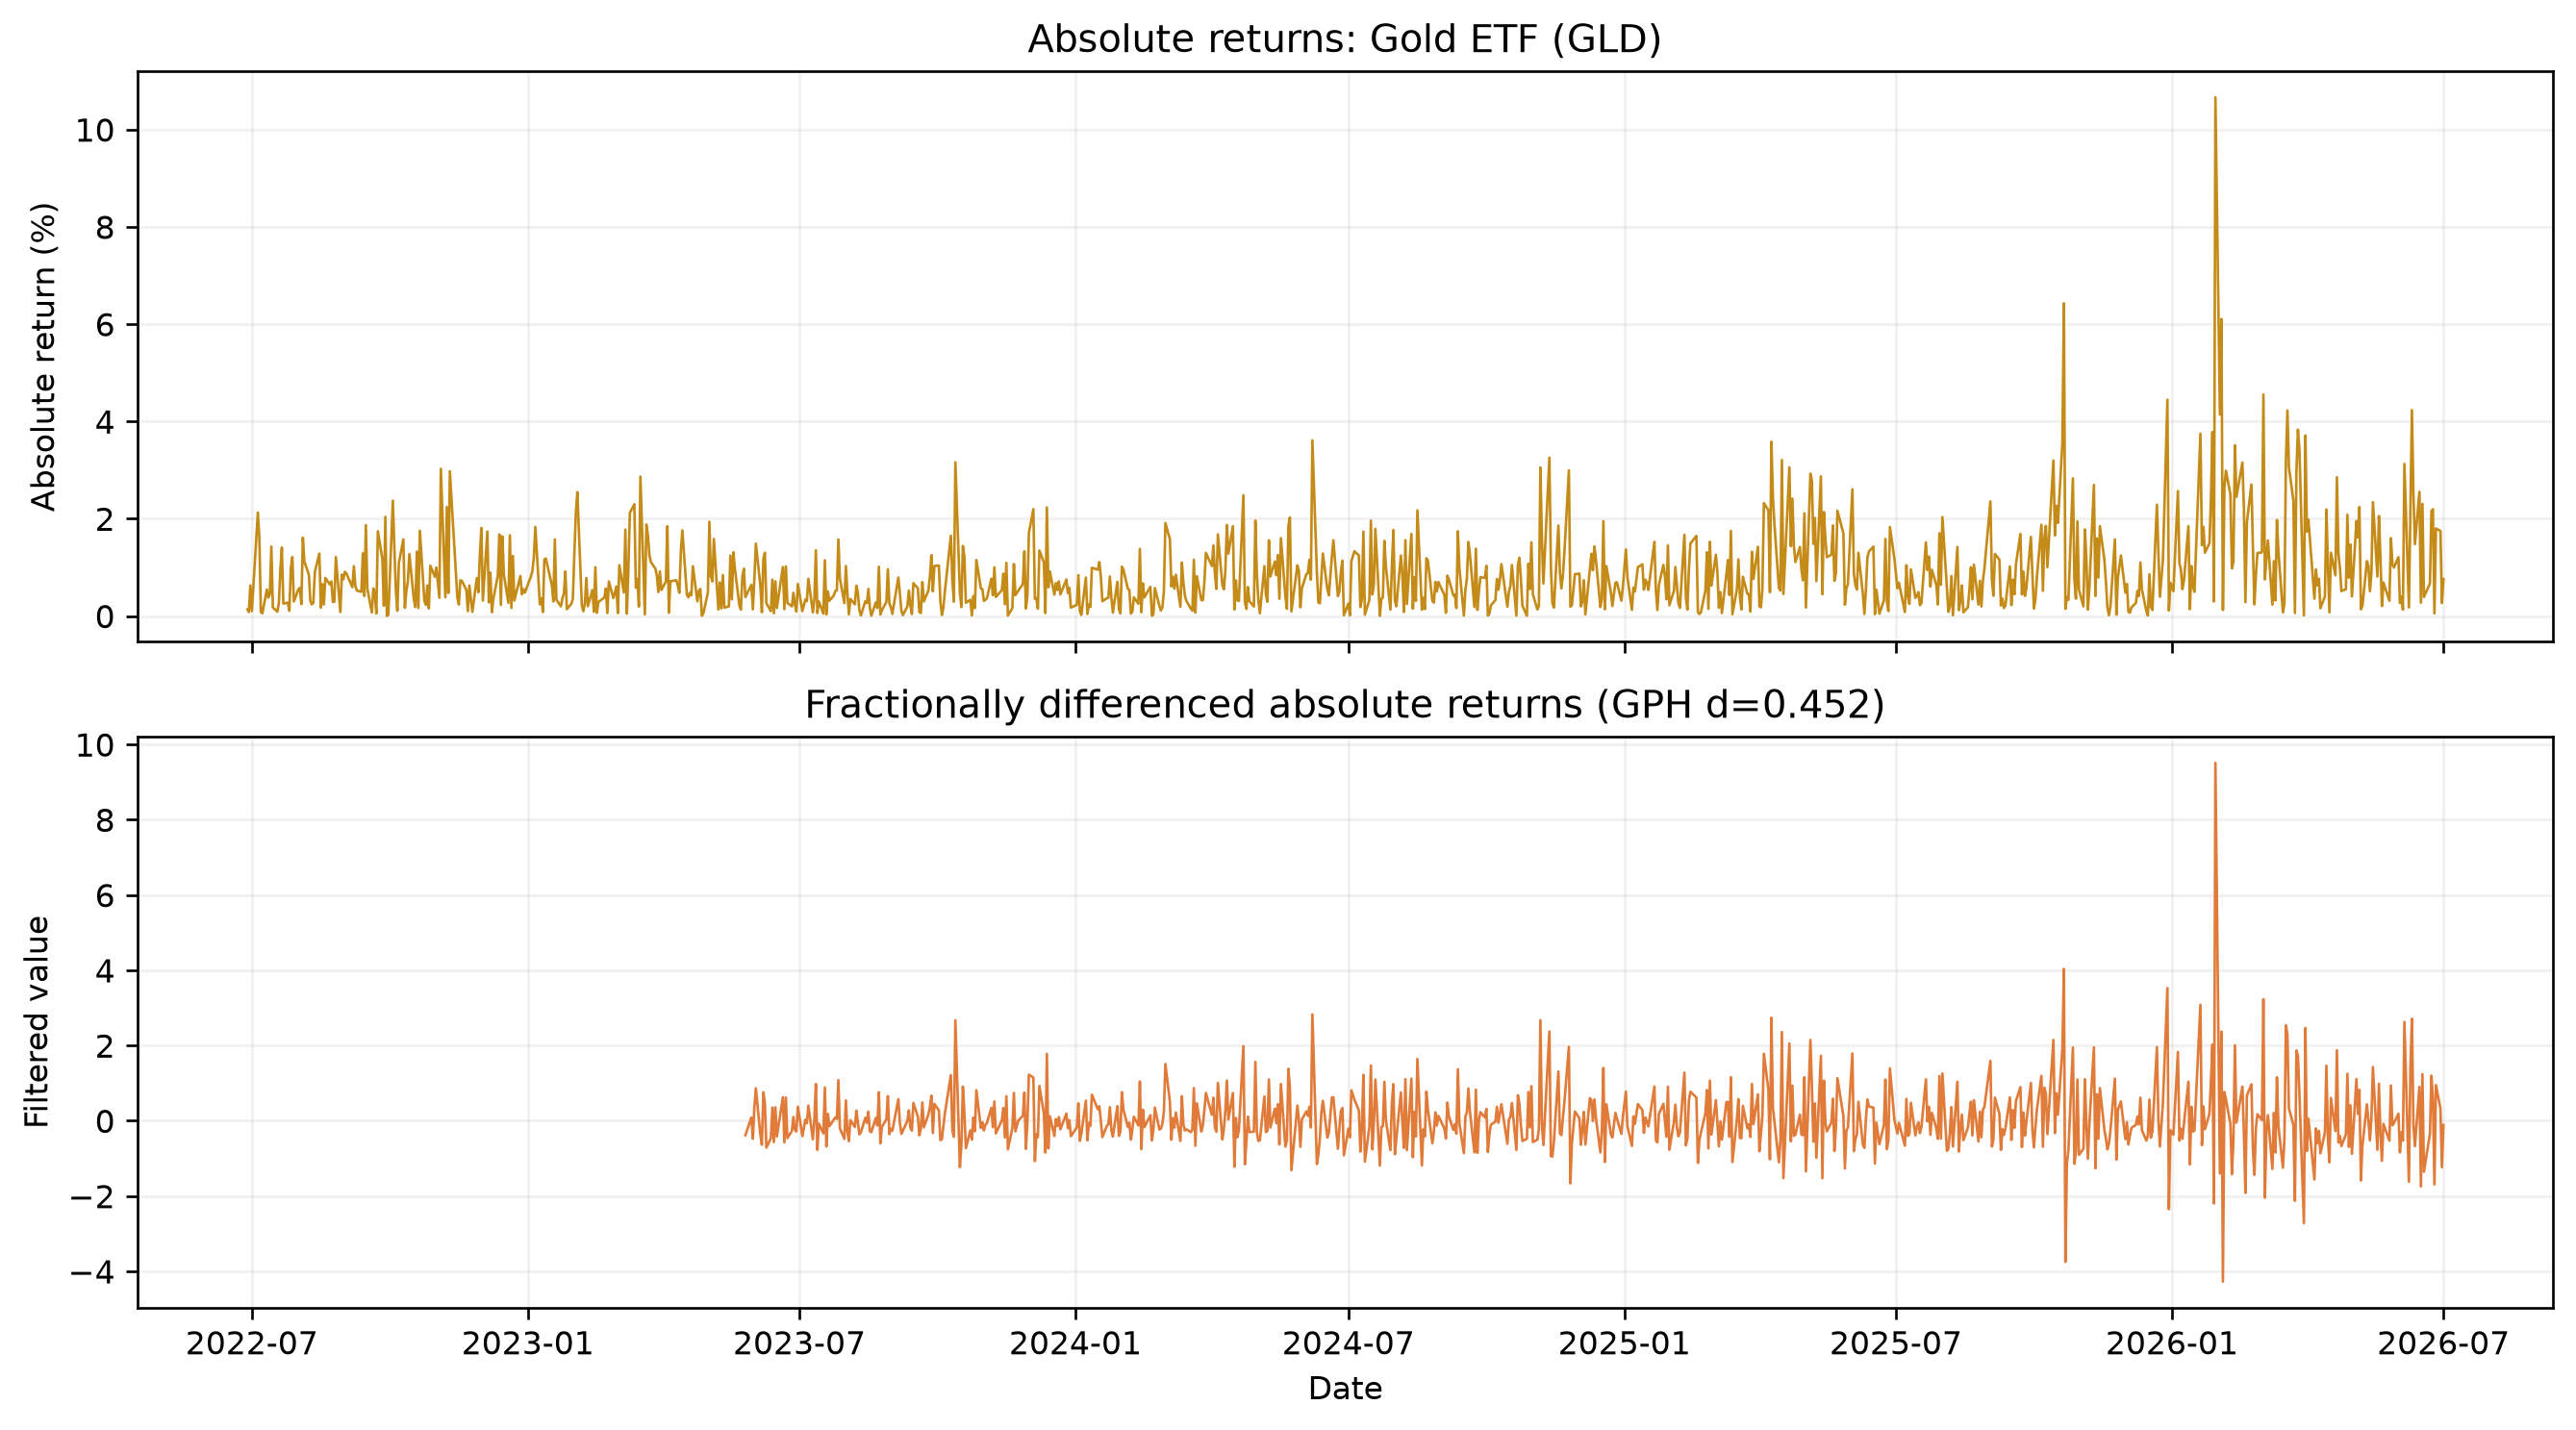
\includegraphics[width=0.86\textwidth]{img/team7_empirical/arfima_fd_gold.png}
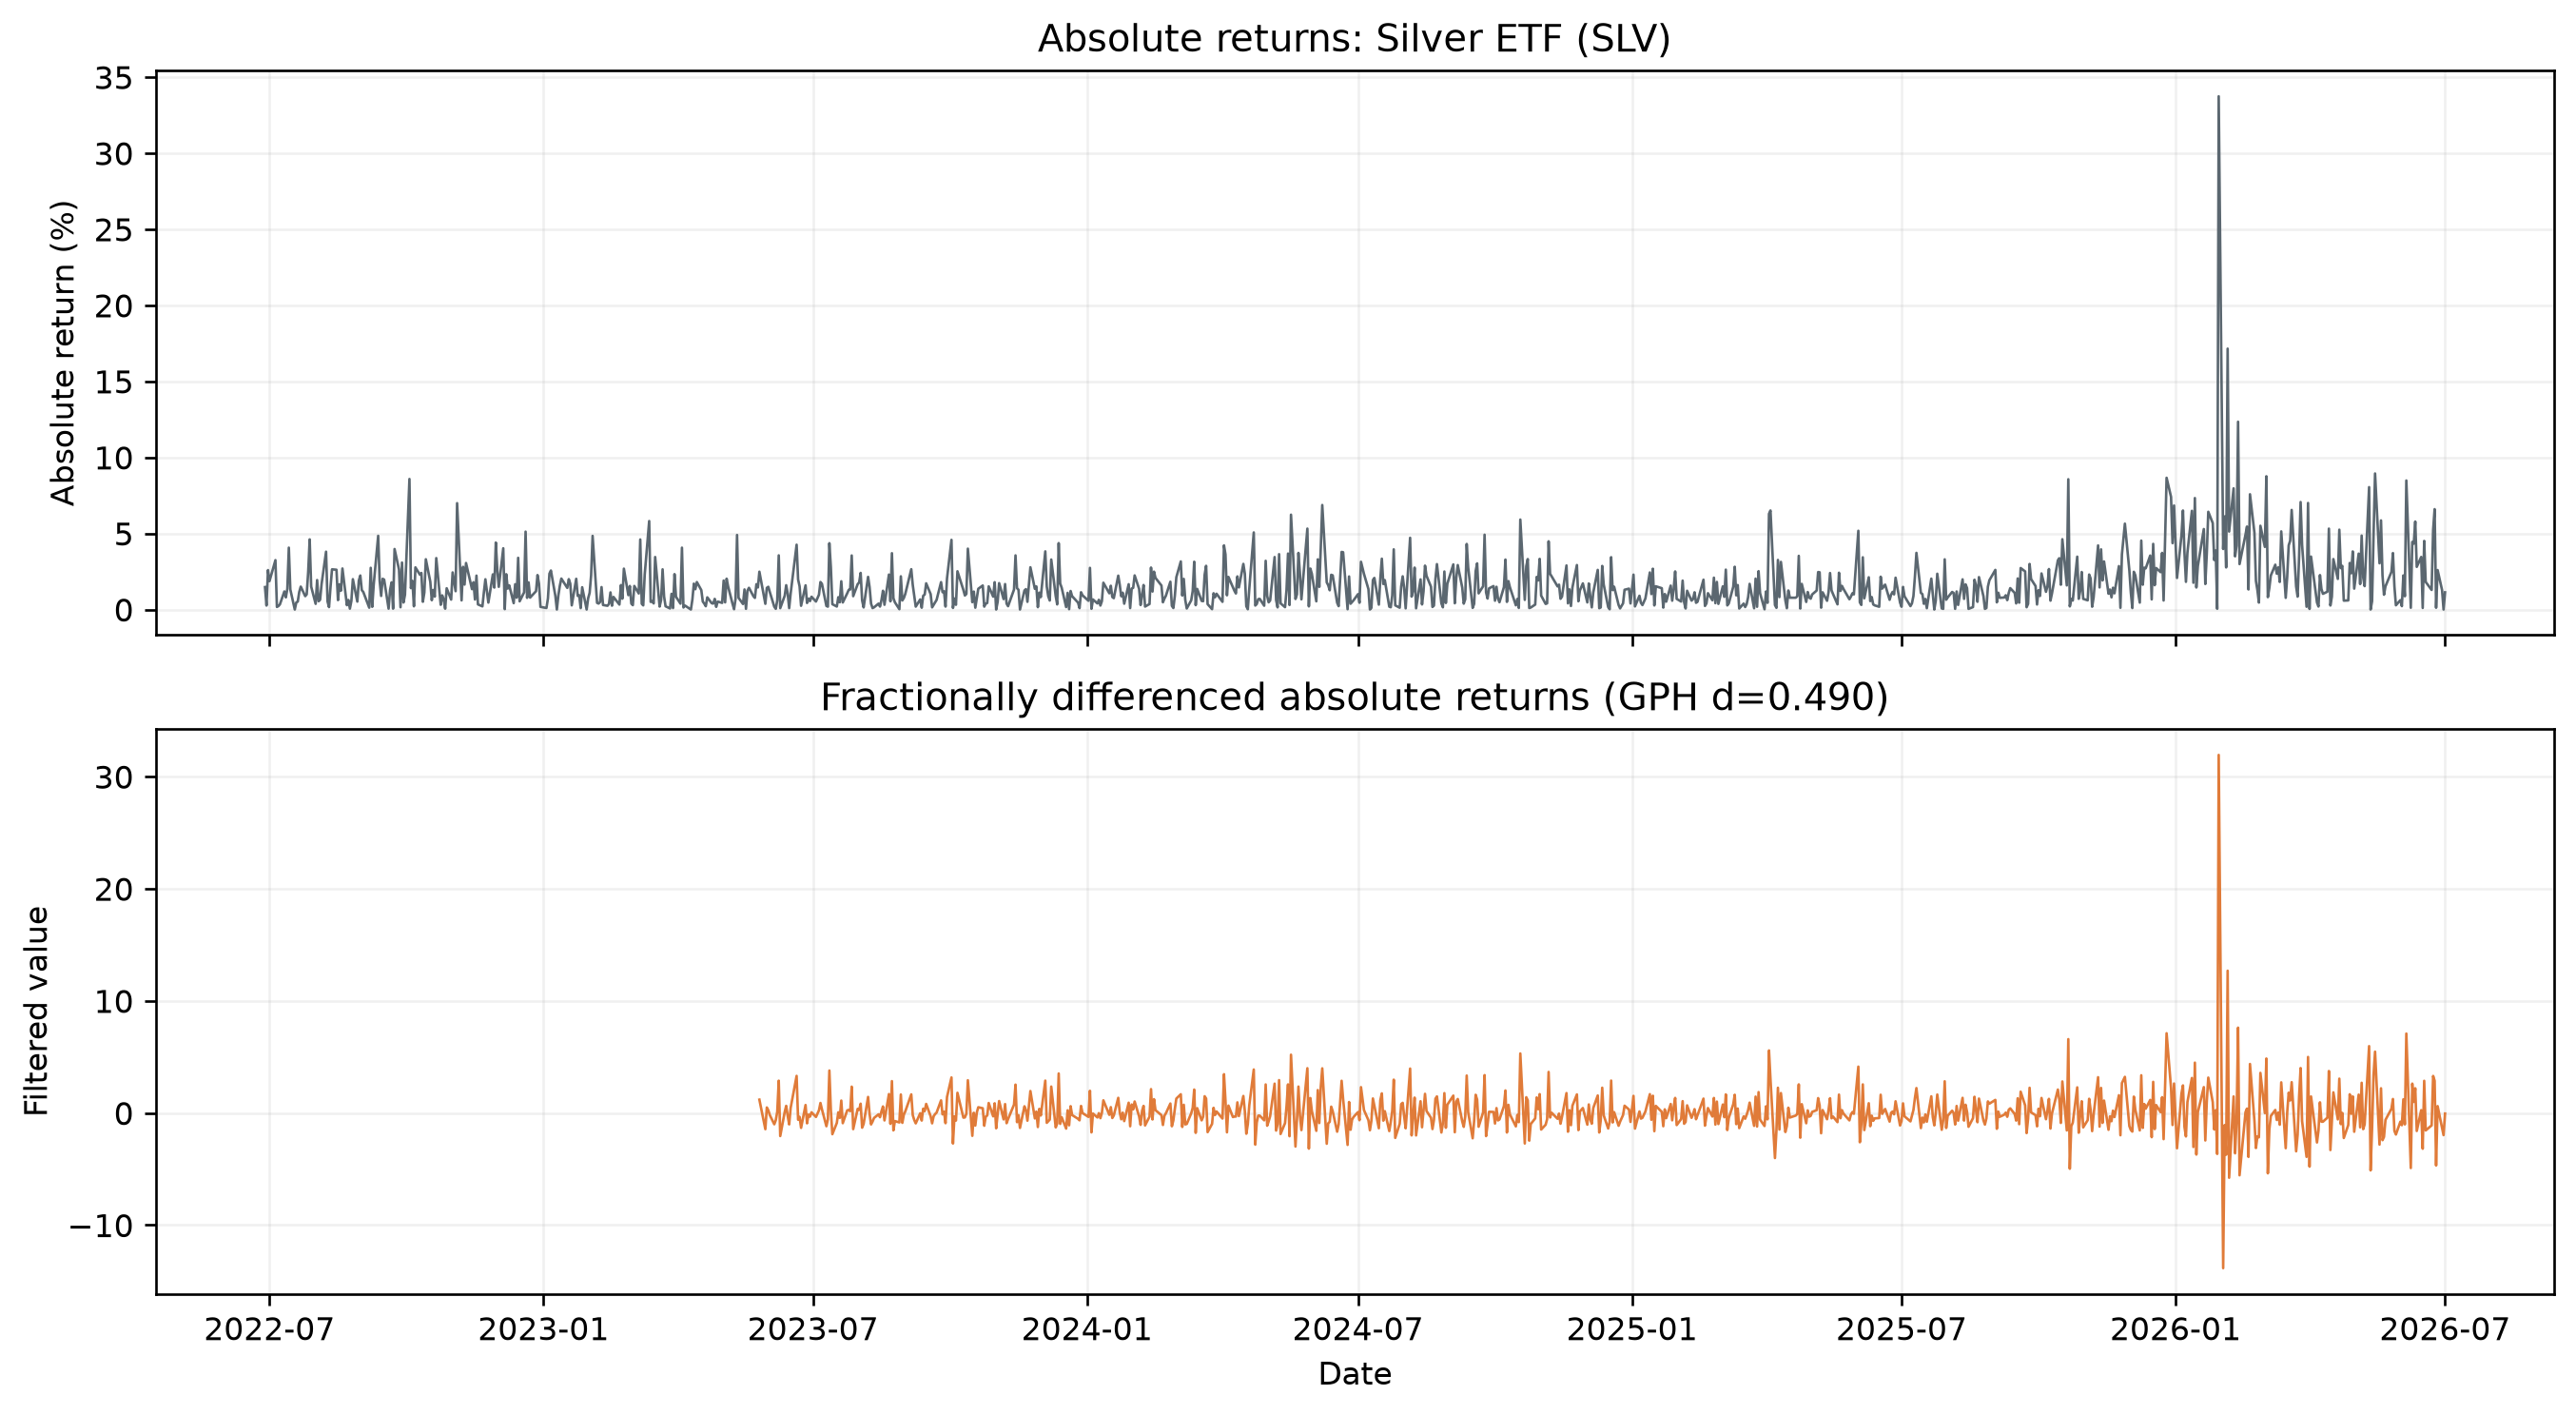
\includegraphics[width=0.86\textwidth]{img/team7_empirical/arfima_fd_silver.png}
\caption{Current LSE absolute returns and fractional filtering; the plotted GPH estimates are 0.452 for GLD and 0.490 for SLV}
\label{fig:t7-fractional-differencing}
\end{figure}

The result requires a stronger qualification than the original standalone
article supplied. In the elementary ARFIMA case, covariance stationarity
requires $d<0.5$; both frozen published point estimates exceed that boundary,
whereas the current LSE estimates lie just below it, with SLV at the imposed
search cap. The evidence is therefore compatible with very strong or
boundary-sensitive persistence, but it does not establish a stable
covariance-stationary ARFIMA law.
Bandwidth sensitivity, alternative long-memory estimators and structural-break
controls remain necessary before assigning a stable economic interpretation.

\clearpage
\section{Limitations and Downstream Resolution}

\paragraph{Limitations of this empirical layer.}
The evidence is conditional on daily frequency and ETF proxies for spot
metals. The chapter deliberately juxtaposes frozen Yahoo tables with current
LSE figures; their estimates are not pooled. Calendar synchronization, the
SPY and DXY-formula proxies, and the use of a yield change alongside asset
returns affect interpretation.
Static and rolling correlations and HC1 regressions are descriptive; they do
not identify monetary, inflationary or geopolitical shocks. Normal-innovation
GARCH does not represent leverage asymmetry, heavy-tailed innovations,
structural breaks or jump arrivals. The GPH result is boundary-sensitive. In
addition, the preserved article tables and repository outputs contain minor
version drift in some AR(1) standard errors; this chapter reports the published
article snapshot and does not disguise it as a fresh recomputation.

\paragraph{Developments already completed in the unified thesis.}
The standalone article described continuous-time stochastic volatility,
option calibration and company valuation as ``next steps.'' They are no
longer future work here. Chapter~8 develops Black--Scholes, Heston,
Bates--Poisson and Bates--Hawkes dynamics, including clustered jumps.
Chapter~9 calibrates the option-pricing layer to a dated GLD surface under the
risk-neutral measure $\mathbb Q$. Chapters~10 and~11 build the production,
cost and DCF interfaces, while Chapters~12 and~13 propagate the four gold-price
engines through a common Barrick valuation experiment and validate their
comparability. The present chapter supplies the historical empirical
motivation for those completed layers; it is not their terminal result.

\paragraph{Residual research agenda.}
Work that remains genuinely open includes a same-date, multi-provider rebuild
of the historical panel; Student-$t$, asymmetric and regime-switching
volatility benchmarks; rolling or expanding-window re-estimation; formal
causal identification of macroeconomic shocks; and robust long-memory tests
under breaks. The most important interface question is the mapping between
historical $\mathbb P$ dynamics and option-implied $\mathbb Q$ parameters.
An augmented filtration that converts textual macroeconomic and geopolitical
information into measurable state variables is also a credible machine-
learning extension, but it is outside the evidence completed in this thesis.

The decision point is therefore precise. ARIMA remains valid for integrated
levels and GARCH remains useful for discrete-time conditional variance, but
low-dimensional historical mean models cannot jointly represent the option
smile, continuous stochastic variance and discontinuous repricing required by
the valuation. Chapter~8 introduces that model layer without treating an
option-implied distribution as an automatic physical-measure forecast.
